\documentclass[11pt]{book}
\usepackage{graphics,graphicx}
\usepackage[auto]{chappg}
%\usepackage[dvips]{graphics,graphicx}
\DeclareGraphicsExtensions{.ps,.jpg,.eps,.pdf,.png}
\usepackage{boxedminipage,amsmath,amsfonts}
\usepackage{url}
%\usepackage{secdot}
%\usepackage{natbib}
\usepackage{verbatim}
%\usepackage{moreverb}
\usepackage{enumerate}
\usepackage{makeidx}
\usepackage{own}
\bibliographystyle{plain}
\makeindex

   

\input{chapters/frontmatter.tex} 
\topmargin 0pt \headheight 14pt \headsep 8pt \textheight 8.6in


\begin{document}

\runcodefalse   % we do not build a manual for folks who only want to run the executables
\uselibsfalse   % we do not build a manual for folks who want to build against the libraries
\developtrue   % we build a manual for folks who want to actively develop code
\bibletrue     % in addition we include stuff that should only be of interest to project managers


%%%%%%%%%%%%%%%%%%%%%%%%%%%%%%%%%%%%%%%%%%
% we can print this bible in regular format (with each chapter starting on a right-hand page)
% or in condensed format (with each chapter starting on a new page, either left or right)
% In the first case, chapters can be printed in isolation and placed into a folder;
% in the second case it is best to print two pages side-by-side on a landscape sheet
%%%%%%%%%%%%%%%%%%%%%%%%%%%%%%%%%%%%%%%%%%
%
\newif\iftwoup
\twoupfalse % regular format --- each chapter starts on a right-hand page 
%\twouptrue % two pages side-by-side in landscape format (paper-conserving) 

\newcommand{\throwpage}{\iftwoup\clearpage\else\cleardoublepage\fi}

%Some cross-referencing index entries (to be expanded as needed)
\index{AMPL Solver Library |see{Third-party software, ASL}}
\index{ASL|see{Third-party software, ASL}}
\index{Blas|see{Third-party software, Blas}}
\index{Harwell Subroutine Library|see{Third-party software, HSL}}
\index{HSL|see{Third-party software, HSL}}
\index{Lapack|see{Third-party software, Lapack}}
\index{Mumps|see{Third-party software, Mumps}}
\index{Bonmin@{\tt Bonmin}|see{COIN-OR projects, {\tt Bonmin}}}
\index{BuildTools@{\tt BuildTools}|see{COIN-OR projects, {\tt BuildTools}}}
\index{Cbc@{\tt Cbc}|see{COIN-OR projects, {\tt Cbc}}}
\index{Cgl@{\tt Cgl}|see{COIN-OR projects, {\tt Cgl}}}
\index{Clp@{\tt Clp}|see{COIN-OR projects, {\tt Clp}}}
%\index{Configuration Manager|see{Microsoft Visual Studio, Configuration Manager}}
\index{Couenne@{\tt Couenne}|see{COIN-OR projects, {\tt Couenne}}}
\index{CppAD@{\tt CppAD}|see{COIN-OR projects, {\tt CppAD}}}
\index{CoinUtils@{\tt CoinUtils}|see{COIN-OR projects, {\tt CoinUtils}}}
%\index{Debug configuration|see{Microsoft Visual Studio, {\tt Debug} configuration}}
\index{DyLP@{\tt DyLP}|see{COIN-OR projects, {\tt DyLP}}}
\index{GLPK@{\tt GLPK}|see{Third-party software, {\tt GLPK}}}
\index{Ipopt@{\tt Ipopt}|see{COIN-OR projects, {\tt Ipopt}}}
\index{nl files|see{AMPL nl format}}
\index{Osi@{\tt Osi}|see{COIN-OR projects, {\tt Osi}}}
%\index{Release configuration|see{Microsoft Visual Studio, {\tt Release} configuration}}
%\index{Release-plus configuration|see{Microsoft Visual Studio, {\tt Release-plus} configuration}}
\index{SYMPHONY@{\tt SYMPHONY}|see{COIN-OR projects, {\tt SYMPHONY}}}
\index{Vol@{\tt Vol}|see{COIN-OR projects, {\tt Vol}}}


\pagenumbering{roman}

\title{Optimization Services \OSstable\ User's Manual (Insider edition)}
\vskip 2in
\author{Horand Gassmann, Jun Ma,  Kipp Martin, and Wayne Sheng}
\maketitle

\chapter*{\centering \begin{normalsize}Abstract\end{normalsize}}
\begin{quotation}
\noindent
This is the extended User's Manual for the Optimization Services (OS) project.  The objective of OS is to provide a
general framework consisting of a set of standards for representing optimization instances, results,
solver options, and communication between clients and solvers in a distributed environment using Web Services.
This COIN-OR\index{COIN-OR} project provides C++ and Java source code for libraries and executable programs that 
implement OS standards.   The OS library includes a robust solver and modeling language interface (API) for linear,
nonlinear and other types of optimization problems.   Also included is the C++ source code for a  command line
executable {\tt OSSolverService}\index{OSSolverService@{\tt OSSolverService}}  for reading problem instances 
(OSiL format\index{OSiL}, nl format\index{AMPL nl format}, MPS format\index{MPS format}) and
calling a solver either locally or on a remote server.  Finally,  both Java\index{Java} source code and a Java {\tt war} 
file are provided for users who wish to set up a solver service on a server running Apache Tomcat\index{Apache Tomcat}.
See the Optimization Services home page {\tt\UrlOs} and the COIN-OR Trac page\index{Trac system} {\tt\UrlTrac} for 
more information.
\end{quotation}
\clearpage


\tableofcontents
\listoffigures
\listoftables

\throwpage

\hyphenation{com-plex-Type}
\hyphenation{GAMS-links}


%\noindent\hrulefill
\throwpage

\pagenumbering{gobble}

\part{Overview}

\pagenumbering{bychapter}

\input{chapters/OSConstitutionArticles.tex}

\input{chapters/Jun_interpretation.tex}

\throwpage

\input{chapters/OSIntro.tex}

\throwpage

\input{chapters/roadmap.tex}



% Part 1 for folks who just want to run the executables

\throwpage

\pagenumbering{gobble}

\part{Running the OS executables}

\pagenumbering{bychapter}

\input{chapters/downloadbinaries.tex}

\throwpage

\input{chapters/OSSolverService.tex}

\throwpage

\input{chapters/OSSolverServiceRules.tex}

\throwpage

\input{chapters/modellang.tex}

\throwpage

\input{chapters/schemadescriptions.tex}


% Part 2 for folks who want to use the libraries to develop their own applications

\throwpage

\pagenumbering{gobble}

\part{Using the OS libraries and API}

\pagenumbering{bychapter}

%\input{chapters/downloadbinaries.tex}

%\throwpage

\division{Code samples to illustrate the OS Project}\label{section:examples}

This chapter describes some sample applications distributed with the OS project. These applications 
are stand-alone developments, but they can be linked against the OS libraries and are intended to show
experienced users how to harness the OS API to build their own interfaces with the OSxL schemas, their private solvers, front ends, or other projects.

\ifdevelop
The example executable files described in this chapter are not part of the regular {\tt configure\rm/\tt make} cycle and are not built by running {\tt configure} and {\tt make}. However, in order to build them, the OS libraries must be installed and available. Each application comes with its own makefile  
and needs to be built separately.

\subdivision{Building the sample applications}\label{section:buildSamples}

Some of these examples (particularly the OSSolverdemo in Section~\ref{section:exampleOSSolverDemo}) 
make use of {\tt Ipopt}\index{COIN-OR projects!Ipopt@{\tt Ipopt}}, which relies on a Fortran compiler\index{Fortran}.
{\bf Windows users} may therefore wish to download a binary distribution and use the solution file {\tt examples.sln} provided there in the 
\begin{verbatim}
examples\MSVisualStudio
\end{verbatim}
directory to build the examples under MS VisualStudio.

\medskip

In order to build the examples in a {\bf unix environment}\index{unix} the user must first run
%
\index{make install@{\tt make install}}
\begin{verbatim}
make install
\end{verbatim}
in the COIN-OS project root directory. (The discussion in this section assumes that the project root directory is
{\tt COIN-OS}.)  Running {\tt make install}  will  place all the header files required by the examples in the directory
\begin{verbatim}
COIN-OS/include
\end{verbatim}
and all of the libraries required by the examples in the directory
\begin{verbatim}
COIN-OS/lib
\end{verbatim}
In addition the folder {\tt pkgconfig} is placed in the {\tt lib} directory as well. Unix must then be informed of the location of this folder as follows:
\begin{verbatim}
export PKG_CONFIG_PATH=<path to pkgconfig directory>
\end{verbatim}
The source code for the examples is in the {\tt COIN-OS/examples} hierarchy.  For instance, the {\tt osModificationDemo}
example of section~\ref{section:exampleOSModDemo} is in the directory
\begin{verbatim}
COIN-OS/examples/osModificationDemo
\end{verbatim}

Next, the user should connect to the appropriate example directory and run {\tt make}.
If the user has done a VPATH\index{VPATH} build, the makefiles\index{makefile|(} will be in each respective example directory under
\begin{verbatim}
vpath_root/examples
\end{verbatim}
otherwise, the makefiles will be in each respective example directory under
\begin{verbatim}
COIN-OS/examples
\end{verbatim}
\else
The binary distribution contains a number of sample applications that illustrate the use of the
OS libraries and other aspects of the OS project. The sample code is found in the {\tt examples}
folder. Each application contains a makefile for unix users; there are also MS Visual Studio project files 
for Windows users. At present only MS Visual Studio 2008 is supported.

Under Windows, connect to the {\tt MSVisualStudio-v9} directory and open {\tt examples.sln} in Visual Studio. All examples can then be built simply by pushing F7 (Build solution). To build only selected examples it is necessary to open the Configuration Manager from the Build menu and select the projects desired to be built.

To build any of the examples under unix, it is at present necessary to set the environment variable
{\tt PKG\_CONFIG\_PATH} to point to the folder {\tt lib/pkgconfig}. Unless some directories were
moved after installing the download, the following unix command will suffice:

\begin{verbatim}
export PKG_CONFIG_PATH=../../lib/pkgconfig
\end{verbatim}

After that, connect to the appropriate directory for the desired project and run {\tt make}. 
For instance, the code and makefile for the {\tt osModDemo}
example of section~\ref{section:exampleOSModDemo} is in the directory
\begin{verbatim}
examples/osModDemo
\end{verbatim}

 
\fi

The {\tt Makefile} in each example directory is fairly simple and is designed to be easily modified 
by the user if necessary.  The part of the {\tt Makefile} to be adjusted, if necessary, is

\begin{verbatim}
##########################################################################
#    You can modify this example makefile to fit for your own program.   #
#    Usually, you only need to change the five CHANGEME entries below.   #
##########################################################################

# CHANGEME: This should be the name of your executable
EXE = OSModDemo
# CHANGEME: Here is the name of all object files corresponding to the source
#           code that you wrote in order to define the problem statement
OBJS =  OSModDemo.o
# CHANGEME: Additional libraries
ADDLIBS =
# CHANGEME: Additional flags for compilation (e.g., include flags)
ADDINCFLAGS =  -I${prefix}/include
# CHANGEME: SRCDIR is the path to the source code; VPATH is the path to
# the executable. It is assumed that the lib directory is in prefix/lib
# and the header files are in prefix/include
SRCDIR = /Users/kmartin/Documents/files/code/cpp/OScpp/COIN-OS/OS/examples/osModDemo
VPATH = /Users/kmartin/Documents/files/code/cpp/OScpp/COIN-OS/OS/examples/osModDemo
prefix = /Users/kmartin/Documents/files/code/cpp/OScpp/vpath
\end{verbatim}


Developers can use the {\tt Makefile}s as a starting point for building applications that use the 
OS project libraries\index{makefile|)}.




\subdivision{Algorithmic Differentiation:  Using the OS Algorithmic Differentiation Methods}\label{section:cppad}

\index{Algorithmic differentiation|(}
In the {\tt examples/algorithmicDiff} folder is test code {\tt OSAlgorithmicDiffTest.cpp}. This code
illustrates the key methods in the {\tt OSInstance}\index{OSInstance@{\tt OSInstance}} API that are used for
algorithmic differentiation.   These methods are described in Section~\ref{section:ad}.



\subdivision{Instance Generator: Using the OSInstance API to Generate Instances}\label{section:exampleOSInstanceGeneration}

This example is found in the {\tt instanceGenerator} folder in the {\tt examples} folder. This example illustrates
how to build a complete in-memory model instance using the {\tt OSInstance}\index{OSInstance@{\tt OSInstance}} API.
See the code {\tt OSInstanceGenerator.cpp} for the complete example. Here we provide a few highlights to illustrate
the power of the API.

The first step is to create an {\tt OSInstance} object.
\begin{verbatim}
OSInstance *osinstance;
osinstance = new OSInstance();
\end{verbatim}

The instance has two variables, $x_{0}$ and $x_{1}$. Variable $x_{0}$ is a continuous variable with lower bound of $-100$ and upper bound of $100$. Variable $x_{1}$ is a binary variable. First declare the instance to have two variables.
\begin{verbatim}
osinstance->setVariableNumber( 2);
\end{verbatim}
Next, add each variable. There is an {\tt addVariable} method with the signature
\begin{verbatim}
addVariable(int index, string name, double lowerBound, double upperBound, char type);
\end{verbatim}
Then the calls for these two variables are
\begin{verbatim}
osinstance->addVariable(0, "x0", -100, 100, 'C');
osinstance->addVariable(1, "x1", 0, 1, 'B');
\end{verbatim}
There is also a method {\tt setVariables} for adding more than one variable simultaneously.  The objective function(s) and constraints are added through similar calls.

Nonlinear terms are also easily added.  The following code illustrates how to add the nonlinear term
$x_{0}*x_{1}$ in the {\tt <nonlinearExpressions>} section of  OSiL. This term is part of constraint~1
and is the second of six expressions contained in the instance.
\begin{verbatim}
osinstance->instanceData->nonlinearExpressions->numberOfNonlinearExpressions = 6;
osinstance->instanceData->nonlinearExpressions->nl = new Nl*[ 6 ];
osinstance->instanceData->nonlinearExpressions->nl[ 1] = new Nl();
osinstance->instanceData->nonlinearExpressions->nl[ 1]->idx = 1;
osinstance->instanceData->nonlinearExpressions->nl[ 1]->osExpressionTree =
new OSExpressionTree();
// the nonlinear expression is stored as a vector of nodes in postfix format
// create a variable nl node for x0
nlNodeVariablePoint = new OSnLNodeVariable();
nlNodeVariablePoint->idx=0;
nlNodeVec.push_back( nlNodeVariablePoint);
// create the nl node for x1
nlNodeVariablePoint = new OSnLNodeVariable();
nlNodeVariablePoint->idx=1;
nlNodeVec.push_back( nlNodeVariablePoint);
// create the nl node for *
nlNodePoint = new OSnLNodeTimes();
nlNodeVec.push_back( nlNodePoint);
// now the expression tree
osinstance->instanceData->nonlinearExpressions->nl[ 1]->osExpressionTree->m_treeRoot =
nlNodeVec[ 0]->createExpressionTreeFromPostfix( nlNodeVec);
\end{verbatim}
\index{Algorithmic differentiation|)}

%\subdivision{Excel:  Using VBA To Generate OSiL}\label{section:exampleExcel}

%\subdivision{Matlab:  Using  MATLAB To Generate OSiL}\label{section:exampleMatlab}

\subdivision{OSModificationDemo: Modifying an In-Memory {\tt OSInstance} Object}\label{section:exampleOSModDemo}

The {\tt osModificationDemo} folder holds the file {\tt OSModificationDemo.cpp}.
This is similar to the {\tt instanceGenerator} example. In this case, a simple
linear program is generated. However, this example also illustrates how to
modify an in-memory OSInstance object. In particular, we illustrate how to
modify an objective function coeffient. Note the repeated occurrence of the code

\begin{verbatim}
solver->osinstance->bObjectivesModified = true;
\end{verbatim}

\noindent in the {\tt OSModificationDemo.cpp} file (lines 175 and 185).
These lines are critical, since otherwise changes made to the OSInstance object
will not be passed to the solver.

This example also illustrates calling a COIN-OR solver,
in this case {\tt Clp}\index{COIN-OR projects!Clp@{\tt Clp}}.

\vskip 8pt

{\bf Important:} the ability to modify a problem instance is still extremely limited in this release.
A better API for problem modification will come with a later release of OS.



\subdivision{OSSolverDemo: Building In-Memory Solver and Option Objects}\label{section:exampleOSSolverDemo}

The code in the  example file {\tt OSSolverDemo.cpp} in the folder {\tt osSolverDemo}  illustrates  how to build solver interfaces and  an in-memory {\tt OSOption} object. In this example we  illustrate building a solver interface and corresponding {\tt OSOption} object for the solvers {\tt Clp}, {\tt Cbc}, {\tt SYMPHONY}, {\tt Ipopt},   {\tt Bonmin}, and {\tt Couenne}.   Each solver class inherits from a virtual {\tt OSDefaultSolver} class. Each solver class has the string data members

\begin{itemize}
\item {\tt osil --} this string conforms to the OSiL standard and holds the model instance.

\item {\tt osol --} this string conforms to the OSoL standard and holds an instance with the 
solver options (if there are any); this string can be empty.

\item {\tt osrl --} this string conforms to the OSrL standard and holds the solution instance; 
each solver interface produces an osrl string.
\end{itemize}

Corresponding to each string there is an in-memory object data member, namely

\begin{itemize}
\item {\tt osinstance --}  an in-memory {\tt OSInstance} object containing the model instance
and {\tt get()} and {\tt set()} methods to access various parts of the model.


\item {\tt osoption --} an in-memory {\tt OSOption} object; solver options can be accessed or 
set using  {\tt get()} and {\tt set()} methods.


\item {\tt osresult --}  an in-memory {\tt OSResult} object; various parts of the model solution  
are accessible through  {\tt get()} and {\tt set()} methods.
\end{itemize}


For each solver we detail five steps:

\begin{itemize}
\item[Step 1:]  Read a model instance from a file  and create the corresponding {\tt OSInstance} object.
For four of the solvers we read a file with the model instance in OSiL format. For the Clp example 
we read an MPS file and convert to OSiL. For the Couenne example we read an AMPL nl file and convert 
to OSiL.

\item[Step 2:]  Create an {\tt OSOption} object and set options appropriate for the given solver.   
This is done by defining

\begin{verbatim}
OSOption* osoption = NULL;
osoption = new OSOption();
\end{verbatim}

A key method in the {\tt OSOption} interface is {\tt setAnotherSolverOption()}.  This method 
takes the following arguments in order.

\begin{itemize}
\item[] {\tt std::string name} -- the option name;
\item[] {\tt std::string value}  -- the value of the option;
\item[] {\tt std::string solver} -- the name of the solver to which the option applies;
\item[] {\tt std::string category} -- options may fall into categories. For example, consider the  
Couenne solver.  This solver is also linked to the Ipopt and Bonmin solvers and  it is possible 
to set options for these solvers through the Couenne API. In order to set an Ipopt option 
you would set the {\tt solver} argument to {\tt couenne} and set the {\tt category} option 
to {\tt ipopt}.

\item[] {\tt std::string type} -- many solvers require knowledge of the data type, so you can set 
the type to {\tt double}, {\tt integer}, {\tt boolean} or {\tt string}, depending on the solver 
requirements. Special types defined by the solver, such as the type {\tt numeric} used by the
Ipopt solver, can also be accommodated. It is the user's responsibility to verify the type
expected by the solver.


\item[] {\tt std::string  description} -- this argument is used to provide any detail or 
additional information about the option.

\item[] Only {\tt name} is mandatory in the OSiL schema. 
However, the API requires mention of all six arguments. 
If any of the remaining optional arguments are not needed, 
an empty string ({\tt""}) should be passed in its place.

\end{itemize}

For excellent documentation that details solver options for Bonmin, Cbc, and Ipopt  we recommend 

\begin{center}
\url{http://www.coin-or.org/GAMSlinks/gamscoin.pdf}
\end{center}


\item[Step 3:] Create the solver object. In the OS project there is a {\it virtual} solver that 
is declared by

\begin{verbatim}
DefaultSolver *solver  = NULL;
\end{verbatim}

The Cbc, Clp and SYMPHONY solvers as well as other solvers of linear and integer linear programs
--- including third-party solvers such as GLPK, Cplex and Gurobi ---  
are all invoked by creating a {\tt CoinSolver().} For example, the following is used to invoke Cbc.

\begin{verbatim}
solver = new CoinSolver();
solver->sSolverName ="cbc";
\end{verbatim}

%Then to declare a specific, for example, an {\tt Ipopt} solver, simply write
Other solvers, particularly Ipopt, Bonmin and Couenne, as well as Csdp where available, 
are implemented separately. So to declare,
for example, an Ipopt solver, one should write

\begin{verbatim}
solver = new IpoptSolver();
solver->sSolverName ="ipopt";
\end{verbatim}

The syntax is the same regardless of solver. 

\item[Step 4:] Import the {\tt OSOption} and {\tt OSInstance} into the solver and solve the model. 
This process is identical regardless of which solver is used. The syntax is:

\begin{verbatim}
solver->osinstance = osinstance;
solver->osoption = osoption;	
solver->solve();
\end{verbatim}

\item[Step 5:] After optimizing the instance,  each of the OS solver interfaces uses the underlying solver API to get the solution result and write the result to a string 
named {\tt osrl} which is a string representing the solution instance in the {\tt OSrL} XML standard.  
This string is accessed by

\begin{verbatim}
solver->osrl
\end{verbatim}


In the example code {\tt OSSolverDemo.cpp} we have written a method,  

\begin{verbatim}
void getOSResult(std::string osrl)
\end{verbatim}

that takes the {\tt osrl} string and creates an {\tt OSResult} object.   
We then illustrate several of the {\tt OSResult} API methods 

\begin{verbatim}
double getOptimalObjValue(int objIdx, int solIdx);
std::vector<IndexValuePair*>  getOptimalPrimalVariableValues(int solIdx);
\end{verbatim}
to get and write out the optimal objective function value, and optimal primal values.  See also Section \ref{section:exampleOSResultDemo}.

\end{itemize}

We now highlight some of the features illustrated by each of the solver examples.

\begin{itemize}
\item {\bf Clp --}  In this example we read in a problem instance in MPS format.  The class 
{\tt OSmps2OS}  has a method {\tt mps2OS} that is used to convert the MPS instance contained 
in a file into an in-memory {\tt OSInstance} object. This example also illustrates how to 
set options using the Osi interface. In particular we turn on intermediate output, which is 
turned off by default in the Coin Solver Interface. 

\item {\bf Cbc --}  In this example we read a problem instance that is in OSiL format and create 
an in-memory {\tt OSInstance} object.  This is quite trivial.  
A  plain-text XML file conforming to the OSiL schema is read into the string {\tt osil}, 
which is then  converted into an in-memory {\tt OSInstance} object by

\begin{verbatim}
OSiLReader *osilreader = NULL;
OSInstance *osinstance = NULL;
osilreader = new OSiLReader(); 
osinstance = osilreader->readOSiL( osil);
\end{verbatim}


We then create an {\tt OSOption} object.   We set the linear programming algorithm to be the primal simplex method and then set the option 
on the pivot selection to be Dantzig rule.  Finally, we set the print level to be 10.

\item {\bf SYMPHONY --}   In this example we also read a problem instance that is in OSiL format and 
create an in-memory {\tt OSInstance} object.  We then create an {\tt OSOption} object and 
illustrate setting the {\tt verbosity} option.

\item {\bf Ipopt --}   In this example we also read a problem instance that is in OSiL format.  
However, in this case we do  not create an {\tt OSInstance} object. We read the OSiL file into 
a string {\tt osil}.  We then feed the {\tt osil} string directly into the Ipopt solver by
\begin{verbatim}
solver->osil = osil;
\end{verbatim} 
The user always has the option of providing the problem instance to the solver 
as either an OSiL string or an in-memory object.

Next we create an {\tt OSOption} object. For Ipopt, we illustrate setting the maximum iteration limit 
and also provide the name of the output file. 
In addition, the {\tt OSOption} object can hold initial solution 
values. We illustrate how to initialize all of the variable to 1.0.

\begin{verbatim}
numVar = 2; //rosenbrock mod has two variables 
xinitial = new double[numVar];
for(i = 0; i < numVar; i++){
    xinitial[ i] = 1.0;
}
osoption->setInitVarValuesDense(numVar, xinitial);
\end{verbatim}



\item {\bf Bonmin --}  In this example we read a problem instance that is in OSiL format and create 
an in-memory {\tt OSInstance} object, just as was done in the Cbc and SYMPHONY examples.   
We then create an {\tt OSOption} object.  In setting the  {\tt OSOption} object we intentionally 
set an option that will cause the Bonmin solver to terminate early.  In particular we set the 
{\tt node\_limit} to zero. 

\begin{verbatim}
osoption->setAnotherSolverOption("node_limit","0","bonmin","","integer","");
\end{verbatim}

This results in early termination of the algorithm. The {\tt OSResult} class API has a method
\begin{verbatim}
std::string getSolutionStatusDescription(int solIdx);
\end{verbatim}

For this example, invoking
\begin{verbatim}
osresult->getSolutionStatusDescription( 0)
\end{verbatim}
gives the result:
\begin{verbatim}
LIMIT_EXCEEDED[BONMIN]: A resource limit was exceeded, we provide the current solution.
\end{verbatim}


\item {\bf Couenne --}   In this example we read in a problem instance in AMPL nl format.  
The class {\tt OSnl2OS}  has a method {\tt nl2OS} that is used to convert the nl instance 
contained in a file into an in-memory {\tt OSInstance} object. This is done as follows:

\begin{verbatim}
// convert to the OS native format
OSnl2OS *nl2osil = NULL;
nl2osil = new OSnl2OS( nlFileName);
// create the first in-memory OSInstance
nl2osil->createOSInstance() ;
osinstance =  nl2osil->osinstance;
\end{verbatim}
\end{itemize}

This part of the example also illustrates setting options in one solver from another. 
Couenne uses Bonmin which uses Ipopt.  So for example,

\begin{verbatim}
osoption->setAnotherSolverOption("max_iter","100","couenne","ipopt","integer","");
\end{verbatim}
identifies the solver as {\tt couenne}, but the value of the fourth argument ({\tt ipopt})  tells the solver 
interface to set the iteration limit on the Ipopt algorithm that is solving the continuous relaxation 
of the problem.  Likewise, the setting
\begin{verbatim}
osoption->setAnotherSolverOption("num_resolve_at_node","3","couenne","bonmin","integer","");
\end{verbatim}
identifies the solver as {\tt couenne}, but the value of the fourth argument ({\tt bonmin})  tells the solver 
interface to tell the Bonmin solver to try three starting points at each node. 

 

\subdivision{OSResultDemo: Building an In-Memory Result Object to Display Solver Results}\label{section:exampleOSResultDemo}

The OS protocol for representing an optimization result is {\tt OSrL}. Like the {\tt OSiL} and {\tt OSoL} protocols, this protocol has an associated in-memory {\tt OSResult} class with corresponding API.  The use of the API is demonstrated in the code {\tt OSResultDemo.cpp} in the folder {\tt OS/examples/OSResultDemo}.  In the code we solve a linear program with the {\tt Clp} solver.  The OS solver interface builds an {\tt OSrL} string that we read into the {\tt OSrLReader} class and create an {\tt OSResult} object. We then use the {\tt OSResult} API to get the optimal primal and dual solution. We also use the API to get the reduced cost values. 


\subdivision{branchCutPrice:  Using Bcp}\label{section:examplebranchCutPrice}

This example illustrates the use of the COIN-OR Bcp (Branch-cut-and-price) project.  
This project provides the user with the ability to have control over each node 
in the branch and bound process. 
This makes it possible to add user-defined cuts and/or user-defined variables. At each node in the tree, 
a call is made to the method {\tt process\_lp\_result()}. In the example problem we illustrate adding 
1)  COIN-OR Cgl cuts, 2) a user-defined cut, and 3) a user-defined variable. 


\subdivision{OSCglCuts: Using the OSInstance API to Generate Cutting Planes}\label{section:exampleOSAddCuts}

In this example, we show how to add cuts to tighten an LP using COIN-OR
{\tt Cgl} (Cut Generation Library)\index{COIN-OR projects!Cgl@{\tt Cgl}}.
A file ({\tt p0033.osil}) in OSiL format is used to create an OSInstance object. The linear programming relaxation
is solved. Then, Gomory, simple rounding, and knapsack cuts are added using {\tt Cgl}.  The model is then optimized
using {\tt Cbc}.

\subdivision{OSRemoteTest:  Calling a Remote Server}\label{section:exampleOSRemoteTest}

This example illustrates the API for the six service methods described in Section~\ref{section:servicemethods}.
The file {\tt osRemoteTest.cpp} in folder {\tt osRemoteTest} first builds a small linear
example, solves it remotely in synchronous mode and displays the solution.
The asynchronous mode is also tested by submitting the problem to a remote solver,
checking the status and either retrieving the answer or killing the process if it has not
yet finished.

{\bf Windows users should note}
that this project links to {\tt wsock32.lib}, which is not part of the Visual Studio  Express Package.  It is necessary
to also download and install the Windows Platform SDK\index{Windows Platform SDK}, which can be found at

\medskip
\noindent{\scriptsize\tt\UrlSdk}. 
\medskip

\ifdevelop
\noindent See also Section~\ref{section:msvs}.
\else
\noindent Further information is provided in the OS User's Manual.
\fi

\subdivision{OSJavaInstanceDemo:  Building an OSiL Instance in
Java}\label{section:exampleOSJavaDemo}
\index{Java|(}

In this example we demonstrate how to build an OSiL instance using the Java
OSInstance API.  The example code also  illustrates calling the {\tt
OSSolverService} executable from Java. In order to use this example, the user should do an svn
checkout:

\begin{verbatim}
svn co https://projects.coin-or.org/svn/OS/branches/OSjava OSjava
\end{verbatim}

The {\tt OSjava} folder contains the file {\tt INSTALL.txt}. Please follow the
instructions in {\tt  INSTALL.txt} under the heading:
\begin{verbatim}
== Install Without a Web Server==
\end{verbatim}

These instructions assume that the user has installed the Eclipse IDE. See
\url{http://www.eclipse.org/downloads/}. At this link we recommend that the 
user get {\tt Eclipse Classic}.  In addition, the user should also have a copy of the
{\tt OSSolverService} executable that is compatible with his or her platform.
The {\tt OSSolverService} executable for several different platforms is
available at \url{http://www.coin-or.org/download/binary/OS/OSSolverService/}. 
The user can also build the executable as described in this Manual.  See Section
\ref{section:build}. 

The code base for this example is in the folder:
\begin{verbatim}
OSjava/OSJavaExamples/src/OSJavaInstanceDemo.java
\end{verbatim}
The code in the file {\tt OSJavaInstanceDemo.java} demonstrates how the
Java OSInstance API that is in {\tt OSCommon} can be used to generate a linear
program and then call the C++ {\tt OSSolverService} executable 
to solve the problem.\index{Java|)}  Running this example in Eclipse will
generate in the folder
\begin{verbatim}
OSjava/OSJavaExamples
\end{verbatim}
two files. It will generate {\tt parincLinear.osil} which is a linear program in
the OSiL format, it will also call the {\tt OSSolverService} executable, which
generates the result file {\tt result.osrl} in the OSrL format. 




\throwpage

\input{chapters/OSDip.tex}

\throwpage

\division{The OS Library Components}\label{section:oslibrary}\index{OSLibrary@{\tt OSLibrary}|(} 

\subdivision{OSAgent}\label{section:osagent}

The {\tt OSAgent}\index{OSAgent@{\tt OSAgent}|(}  part of the library is used to facilitate communication
with remote solvers. It is not used if the solver is invoked locally (i.e., on the same machine).
There are two key classes in the {\tt OSAgent} component of the OS library. The two classes are
{\tt OSSolverAgent}\index{OSSolverAgent@{\tt OSSolverAgent}} and {\tt WSUtil}\index{WSUtil@{\tt WSUtil}}.

The {\tt OSSolverAgent} class is used to contact a remote solver service.  For example, assume that {\tt sOSiL}
is a string with a problem instance and {\tt sOSoL} is a string with solver options. Then the following code
will call a solver service and invoke the {\tt solve} method.
\begin{verbatim}
OSSolverAgent *osagent;
string serviceLocation = "http://xxx.xxx.xxx.xxx:8080/OSServer/services/OSSolverService";
osagent = new OSSolverAgent(  serviceLocation );
string sOSrL = osagent->solve(sOSiL, sOSoL);
\end{verbatim}
(The string `{\tt xxx.xxx.xxx.xxx}' must be replaced by the IP address of a computer running the {\tt OSSolverService}.)
Other methods in the {\tt OSSolverAgent} class are {\tt send}, {\tt retrieve}, {\tt getJobID}, {\tt knock}, and {\tt kill}.  
The use of these methods is described in Section~\ref{section:servicemethods}.



The methods in the {\tt OSSolverAgent} class call methods in the {\tt WSUtil} class that perform such tasks as 
creating and parsing SOAP messages and making low level socket calls to the server running the solver service. 
The average user will not use methods in the {\tt WSUtil} class, but they are available to anyone wanting to make socket calls or create SOAP messages.

\iffalse
There is also a method, {\tt OSFileUpload}, in the OSAgentClass that is used to upload files from the hard drive of a client to the server. 
It is very fast and does not involve SOAP or Web Services. The {\tt OSFileUpload}  method is illustrated and described in the example code 
{\tt OSFileUpload.cpp} described in Section~\ref{section:fileupload}.
\index{OSAgent@{\tt OSAgent}|)}
\fi

\subdivision{OSCommonInterfaces}

The classes in the OSCommonInterfaces component of the OS library are used to read and write files and strings
in the OSiL and OSrL protocols. See Section~\ref{section:schemadescriptions} for more detail on OSiL, OSrL,
and other OS protocols. For a complete listing of all of the files in {\tt OSCommonInterfaces} see the 
Doxygen\index{Doxygen} documentation we deposited at {\tt\UrlDoxygen}. Users who have 
Doxygen installed on their system can also create their own version of the documentation 
(see \ifdevelop Section~\ref{section:documentation}\else the OS Users' Manual\fi). 
Below we highlight some key classes.





\subsubdivision{The OSInstance Class}\label{section:osinstanceclass}

The OSInstance\index{OSInstance@{\tt OSInstance}|(} class is the in-memory representation of an optimization instance and is a key
class for users of the OS project. This class has an API defined by a collection of {\tt get()} methods for
extracting various components (such as bounds and coefficients) from a problem instance, a collection of
{\tt set()} methods for modifying or generating an optimization instance, and a collection of {\tt calculate()}
methods for function, gradient, and Hessian evaluations.  See Section~\ref{section:osinstanceAPI}.
We now describe how to create an {\tt OSInstance} object and the close relationship between the OSiL\index{OSiL} schema
and the {\tt OSInstance} class.

\subsubdivision{Creating an {\tt OSInstance} Object}

The OSCommonInterfaces component contains an {\tt OSiLReader}  class for reading an instance in an OSiL string and
creating an in-memory {\tt OSInstance} object.  Assume that {\tt sOSiL} is a string that will hold the instance in OSiL format. Creating an {\tt OSInstance} object is illustrated in Figure~\ref{figure:creatingosinstanceobject}.

\begin{figure}[ht]
\centering
   \small {\obeyspaces\let =\
\fbox{\tt\begin{tabular}{@{}l@{}}
OSiLReader *osilreader = NULL;\\[\Sb]
OSInstance *osinstance = NULL;\\[\Sb]
osilreader = new OSiLReader();\\[\Sb]
osinstance = osilreader->readOSiL( sOSiL);\\[\Sb]
\end{tabular} }} \bigskip
\caption{Creating an {\tt OSInstance} Object} \label{figure:creatingosinstanceobject}
\end{figure}

\subsubdivision{Mapping Rules}\label{section:mappingrules}

The {\tt OSInstance} class has two members, {\tt instanceHeader} and {\tt instanceData}.  
These correspond to the XML elements {\tt <instanceHeader>} and {\tt <instanceData>}.
They are of type {\tt InstanceHeader} and {\tt InstanceData}, respectively, which in turn  
correspond to the OSiL schema's complexTypes {\tt InstanceHeader} and {\tt InstanceData}, and 
in themselves are C++ classes.

    Moving down one level, Figure~\ref{figure:instancedata} shows that the {\tt InstanceData} class has in turn 
the members {\tt variables}, {\tt objectives}, {\tt constraints}, {\tt linearConstraintCoefficients}, 
{\tt quadraticCoefficients}, and {\tt nonlinearExpressions}, corresponding to the respective elements 
in the OSiL file that have the same name. Each of these are instances of associated classes which correspond
to complexTypes in the OSiL schema.


\begin{figure}[ht]
\centering
   \small {\obeyspaces\let =\
\fbox{\tt\begin{tabular}{@{}l@{}}
class OSInstance\{\\[\Sb]
public:\\[\Sb]
     OSInstance(); \\[\Sb]
     InstanceHeader *instanceHeader;\\[\Sb]
     InstanceData *instanceData;    \\[\Sb]
\}; //class OSInstance\\[\Sb]
\end{tabular} }} \bigskip
\caption{The {\tt OSInstance} class} \label{figure:osinstance}
\end{figure}


\begin{figure}[ht]
\centering
   \small {\obeyspaces\let =\
\fbox{\tt\begin{tabular}{@{}l@{}}
class InstanceData\{\\[\Sb]
public:\\[\Sb]
     InstanceData();\\[\Sb]
     Variables *variables;\\[\Sb]
     Objectives *objectives;\\[\Sb]
     Constraints *constraints;\\[\Sb]
     LinearConstraintCoefficients *linearConstraintCoefficients;\\[\Sb]
     QuadraticCoefficients *quadraticCoefficients;\\[\Sb]
     NonlinearExpressions *nonlinearExpressions;\\[\Sb]
\}; // class InstanceData
\end{tabular} }} \bigskip
\caption{The {\tt InstanceData} class} \label{figure:instancedata}
\end{figure}


\begin{figure}[hb]
%\includegraphics[scale=0.8]{../../figures/paradigm1.eps}
\centering
   \scriptsize {\obeyspaces\let =\
\fbox{\tt\begin{tabular}{@{}l@{}}
\textsf{\textbf{Schema complexType  \hspace{3.64in}  In-memory class}}\\[\Sa]
<xs:complexType name="Variables">  <-------------------------------------------->  class Variables\{\\[\Sb]
                                                                                   public:\\[\Sb]
  <xs:sequence>                                                                      Variables();\\[\Sb]
    <xs:element name="var" type="Variable" maxOccurs="unbounded"/>  <----------->    Variable *var;\\[\Sb]
  </xs:sequence>                                                                   \\[\Sb]
  <xs:attribute name="numberOfVariables" type="xs:nonnegativeInteger"                 \\[\Sb]
                use="required"/>  <--------------------------------------------->    int numberOfVariables;\\[\Sb]
</xs:complexType>                                                                  \}; // class Variables\\[\Sb]
 \\[\Sb]
 \\[\Sb]
<xs:complexType name="Variable">  <--------------------------------------------->  class Variable\{\\[\Sb]
                                                                                   public:\\[\Sb]
                                                                                     Variable();\\[\Sb]
  <xs:attribute name="name" type="xs:string" use="optional"/>  <---------------->    string name;\\[\Sb]
  <xs:attribute name="type" use="optional" default="C">  <---------------------->    char type;\\[\Sb]
    <xs:simpleType>\\[\Sb]
      <xs:restriction base="xs:string">\\[\Sb]
        <xs:enumeration value="C"/>\\[\Sb]
        <xs:enumeration value="B"/>\\[\Sb]
        <xs:enumeration value="I"/>\\[\Sb]
        <xs:enumeration value="S"/>\\[\Sb]
        <xs:enumeration value="D"/>\\[\Sb]
        <xs:enumeration value="J"/>\\[\Sb]
      </xs:restriction>\\[\Sb]
    </xs:simpleType>\\[\Sb]
  </xs:attribute>\\[\Sb]
  <xs:attribute name="lb" type="xs:double" use="optional" default="0"/>  <------>    double lb;\\[\Sb]
  <xs:attribute name="ub" type="xs:double" use="optional" default="INF"/>  <---->    double ub;\\[\Sb]
</xs:complexType>                                                                  \}; // class Variable\\[\Sb]
 \\[\Sb]
 \\[\Sb]
\textsf{\textbf{OSiL elements          \hspace{1.83in}  In-memory objects}}\\[\Sa]
<variables numberOfVariables="2">                   OSInstance *osinstance;\\[\Sb]
   <var lb="0" name="x0" type="C"/>                 osinstance->instanceData->variables->numberOfVariables=2;\\[\Sb]
   <var lb="0" name="x1" type="C"/>                 osinstance->instanceData->variables->var=new Variable*[2];\\[\Sb]
</variables>                                        osinstance->instanceData->variables->var[0]->lb=0;\\[\Sb]
                                                    osinstance->instanceData->variables->var[0]->name="x0";\\[\Sb]
                                                    osinstance->instanceData->variables->var[0]->type={\rm 'C'};\\[\Sb]
                                                    osinstance->instanceData->variables->var[1]->lb=0;\\[\Sb]
                                                    osinstance->instanceData->variables->var[1]->name="x1";\\[\Sb]
                                                    osinstance->instanceData->variables->var[1]->type={\rm 'C'};
\end{tabular} }} \medskip\\[\Sb]
\caption{The {\tt <variables>} element as an {\tt OSInstance} object} \label{figure:osinstancevariables}
\end{figure}


Figure~\ref{figure:osinstancevariables} uses the {\tt Variables} class to provide a closer look 
at the correspondence between schema and class. On the right, the {\tt Variables} class contains 
the data member {\tt numberOfVariables} and a pointer to the object {\tt var} of class {\tt Variable}. 
The {\tt Variable} class has  data members {\tt lb} (double), {\tt ub} (double), {\tt name} (string), 
and {\tt type} (char). On the left the corresponding XML {\tt complexType}s are shown, with arrows indicating 
the correspondences. The following rules describe the mapping between the OSiL schema and the 
{\tt OSInstance} class. 
(In order to facilitate the mapping, we insist in the schema construction that every {\tt complexType} be named, 
even though this is not strictly necessary in XML.)
%
\begin{itemize}

\item  Each {\tt complexType} in an OSiL schema corresponds to a class in {\tt OSInstance}.
Thus the OSiL schema's {\tt complexType} {\tt Variables} corresponds to {\tt OSInstance}'s class {\tt Variables}.
Elements in an actual XML file then correspond to objects in {\tt OSInstance};
for example, the {\tt <variables>} element that is of type {\tt Variables} in an OSiL file
corresponds to a {\tt variables} object in {\tt OSInstance}. 
%(Since {\tt <variables>} is an element of the
%element {\tt <instanceData>} in OSiL, the {\tt variables} object is contained in class {\tt instanceData}.)

\item An attribute or element used in the definition of a {\tt complexType} is a member of the 
corresponding {\tt OSInstance} class, and the type of the attribute or element matches the type 
of the member.  In Figure~\ref{figure:osinstancevariables}, for example, {\tt lb} is an attribute 
of the OSiL {\tt complexType} named {\tt Variable}, and {\tt lb} is a member of the {\tt OSInstance} 
class {\tt Variable}; both have type {\tt double}.  Similarly, {\tt <var>} is an element in the definition 
of the OSiL {\tt complexType} named {\tt Variables}, and {\tt var} is a member of the {\tt OSInstance} 
class {\tt Variables}; the {\tt <var>} element has type {\tt Variable} and the {\tt var} member is a 
{\tt Variable} object.

\item A schema sequence corresponds to an array. For example, in Figure~\ref{figure:osinstancevariables} the complexType {\tt Variables} has a sequence of {\tt <var>} elements that are of type {\tt Variable}, and the corresponding {\tt Variables} class has a member that is an array of type {\tt Variable}.

\item
XML allows a wide range of data subtypes, which do not always have counterparts in the {\tt OSInstance} object.
For instance, the attribute {\tt type} in the {\tt <var>} element forms an enumeration, while the corresponding
member of the {\tt Variable} class is declared as {\tt char}. 

\item
XML allows default values for optional attributes; these default values can be set inside of the constructor of the corresponding data member. 
\end{itemize}
%
General nonlinear terms are stored in the data structure as {\tt OSExpressionTree} objects, which are the subject of the next section.

     The {\tt OSInstance} class has a collection of {\tt get()}, {\tt set()}, and {\tt calculate()} methods 
that act as an API for the optimization instance and are described in Section~\ref{section:osinstanceAPI}.




\subsubdivision{The OSExpressionTree OSnLNode Classes}\label{section:osexpressiontreeclass}

The {\tt OSExpressionTree}\index{OSExpressionTree@{\tt OSExpressionTree}} class provides the in-memory representation
of the nonlinear terms.  Our design goal is  to allow for efficient parsing of OSiL\index{OSiL} instances,
while providing an API that meets the needs of diverse solvers.  Conceptually, any nonlinear expression in the
objective or constraints is represented by a tree.  The expression tree for the nonlinear part of the
objective function~(\ref{eq:roobj}), for example, has the form illustrated in Figure~\ref{figure:expressiontree}.
The choice of a data structure to store such a tree --- along with the associated methods of an API --- is a key aspect
in the design of the {\tt OSInstance} class.

\begin{figure}[ht]
\centering
%\includegraphics[scale=0.38]{\figurepath/expressiontree.png}
\includegraphics[scale=0.38]{./figures/expressiontree.png}
\caption{Conceptual expression tree for the nonlinear part of the objective (\ref{eq:roobj}).}\label{figure:expressiontree}
\end{figure}


A base abstract class {\tt OSnLNode} is defined and  all of an OSiL file's
operator and operand elements used in defining a
nonlinear expression are extensions of the base element type {\tt OSnLNode}. There is an element type {\tt OSnLNodePlus}, 
for example, that extends {\tt OSnLNode}; then in an OSiL instance file, there are {\tt <plus>} elements that 
are of type {\tt OSnLNodePlus}.   Each {\tt OSExpressionTree} object contains a pointer to an {\tt OSnLNode} object 
that is the root of the corresponding expression tree.  To every element that extends the {\tt OSnLNode} type in an 
OSiL instance file, there corresponds a class that derives from the {\tt OSnLNode} class in an {\tt OSInstance} 
data structure.  Thus we can construct an expression tree of homogenous nodes, and methods that operate on the 
expression tree to calculate function values, derivatives, postfix notation, and the like do not require switches 
or complicated logic.


\begin{figure}[ht]
\centering
   \small {\obeyspaces\let =\
\fbox{\tt\begin{tabular}{@{}l@{}}
   double OSnLNodePlus::calculateFunction(double *x)\{\\[\Sb]
      m\_dFunctionValue = \\[\Sb]
         m\_mChildren[0]->calculateFunction(x) +\\[\Sb]
         m\_mChildren[1]->calculateFunction(x);\\[\Sb]
      return m\_dFunctionValue;\\[\Sb]
   \} //calculateFunction\\[\Sb]
\end{tabular} }} \medskip
\caption{The function calculation method for the {\tt plus} node class with polymorphism}
   \vspace{-8pt} \label{figure:calcfunction}
\end{figure}


The {\tt OSInstance} class has a variety of {\tt calculate()} methods, based on two pure virtual functions 
in the {\tt OSInstance} class.  The first of these, {\tt calculateFunction()}, takes an array of {\tt double} 
values corresponding to decision variables, and evaluates the expression tree for those values.  Every class
that extends {\tt OSnLNode} must implement this method.  As an example, the {\tt calculateFunction} method 
for the {\tt OSnLNodePlus} class is shown in Figure~\ref{figure:calcfunction}.  Because the OSiL instance 
file must be validated against its schema, and in the schema each {\tt <OSnLNodePlus>} element is specified 
to have exactly two child elements, this {\tt calculateFunction} method can assume that there are exactly 
two children of the node that it is operating on.  The use of polymorphism and recursion makes adding new 
operator elements easy; it is simply a matter of adding a new class and implementing the {\tt calculateFunction()} 
method for it.



Although in the OSnL schema, there are 200+ nonlinear operators, only the following {\tt  OSnLNode} classes are currently supported in our implementation.

\begin{itemize}
\item OSnLNodeVariable
\item OSnLNodeTimes
\item OSnLNodePlus
\item OSnLNodeSum
\item OSnLNodeMinus
\item OSnLNodeNegate
\item OSnLNodeDivide
\item OSnLNodePower
\item OSnLNodeProduct
\item OSnLNodeLn
\item OSnLNodeSqrt
\item OSnLNodeSquare
\item OSnLNodeSin
\item OSnLNodeCos
\item OSnLNodeExp
\item OSnLNodeIf
\item OSnLNodeAbs
\item OSnLNodeMax
\item OSnLNodeMin
\item OSnLNodeE
\item OSnLNodePI
\item OSnLNodeAllDiff
\end{itemize}
\index{OSInstance@{\tt OSInstance}|)}



\subsubdivision{The OSOption Class}\label{section:osoptionclass}

The {\tt OSOption}\index{OSOption@{\tt OSOption}|(} class is the in-memory representation of the options 
associated with a particular optimization task. It is another key
class for users of the OS project. This class has an API defined by a collection of {\tt get()} methods for
extracting various components (such as initial values for decision variables, solver options, job parameters, etc.), 
and a collection of {\tt set()} methods for modifying or generating an option instance. The relationship between
in-memory classes and objects on one hand and complexTypes and elements of the OSoL schema follow the same mapping rules
laid out in Section~\ref{section:mappingrules}.
\index{OSOption@{\tt OSOption}|)}

\subsubdivision{The OSResult Class}\label{section:osresultclass}

Similarly the {\tt OSResult}\index{OSResult@{\tt OSResult}|(} class is the in-memory representation of the 
results returned by the solver and other information associated with a particular optimization task. 
This class has an API defined by a collection of {\tt set()} methods that allow a solver to create a result instance
and a collection of {\tt get()} methods for
extracting various components (such as optimal values for decision variables, optimal objective function value, 
optimal dual variables, etc.). The relationship between
in-memory classes and objects on one hand and complexTypes and elements of the OSoL schema follow the same 
mapping rules laid out in Section~\ref{section:mappingrules}.
\index{OSResult@{\tt OSResult}|)}



\subdivision{OSModelInterfaces}\label{section:osmodelinterfaces}

This part of the OS library is designed to help integrate the OS standards with other standards and modeling systems.

\subsubdivision{Converting MPS Files}

The MPS standard\index{MPS format|(} is still a popular format for representing linear and integer programming problems.
In {\tt OSModelInterfaces,} there is a class {\tt OSmps2osil}\index{OSmps2osil@{\tt OSmps2osil}|(} that can be used
to convert files in MPS format into the OSiL\index{OSiL} standard. It is used as follows.

\begin{verbatim}
OSmps2osil *mps2osil = NULL;
DefaultSolver *solver  = NULL;
solver = new CoinSolver();
solver->sSolverName = "cbc";
mps2osil = new OSmps2osil(  mpsFileName);
mps2osil->createOSInstance() ;
solver->osinstance = mps2osil->osinstance;
solver->solve();
\end{verbatim}

The {\tt OSmps2osil} class constructor takes a string which should be the
file name of the instance in MPS format. The constructor then uses the
{\tt CoinUtils}\index{COIN-OR projects!CoinUtils@{\tt CoinUtils}} library to read and parse the MPS file.  The class method {\tt createOSInstance} then builds  an in-memory {\tt osinstance} object  that can be used by a solver.
\index{OSmps2osil@{\tt OSmps2osil}|)}\index{MPS format|)}

\subsubdivision{Converting AMPL nl Files}\label{section:nl2osil}

AMPL is a popular modeling language that saves  model instances in the AMPL nl format\index{AMPL nl format|(}.
The {\tt OSModelInterfaces} library provides a class, {\tt OSnl2osil}\index{OSnl2osil@{\tt OSnl2osil}},
for reading an nl file and creating a
corresponding in-memory  {\tt osinstance}\index{OSInstance@{\tt OSInstance}} object. It is used as follows.

\begin{verbatim}
OSnl2osil *nl2osil = NULL;
DefaultSolver *solver  = NULL;
solver = new LindoSolver();
nl2osil = new OSnl2osil( nlFileName);
nl2osil->createOSInstance() ;
solver->osinstance = nl2osil->osinstance;
solver->solve();
\end{verbatim}


The {\tt OSnl2osil} class works much like the {\tt OSmps2osil}\index{OSmps2osil@{\tt OSmps2osil}} class. The
{\tt OSnl2osil} class constructor takes a string which should be the file name of the instance in nl format. The constructor then uses the AMPL ASL library routines to read and parse the nl file. The class method {\tt createOSInstance} then builds  an in-memory {\tt osinstance} object  that can be used by a solver.

In Section~\ref{section:amplclient}  we describe the {\tt OSAmplClient}\index{OSAmplClient@{\tt OSAmplClient}}
executable that acts as a ``solver'' for AMPL. The {\tt OSAmplClient} uses the {\tt OSnl2osil} class to convert
the instance in nl format to OSiL\index{OSiL} format before calling a solver either locally or remotely.
\index{AMPL nl format|)}


\subdivision{OSParsers}\label{section:osparsers}

The OSParsers component of the OS library contains reentrant parsers that  read OSiL\index{OSiL|(},
OSoL\index{OSoL} and OSrL\index{OSrL} strings and build, respectively, in-memory 
OSInstance\index{OSInstance@{\tt OSInstance}}, OSOption\index{OSOption@{\tt OSOption}} and 
OSResult\index{OSResult@{\tt OSResult}}  objects.


The OSiL parser is invoked through an {\tt OSiLReader} object as illustrated below. Assume {\tt osil} is a string with the problem instance.
\begin{verbatim}
OSiLReader *osilreader = NULL;
OSInstance *osinstance = NULL;
osilreader = new OSiLReader();
osinstance = osilreader->readOSiL( osil);
\end{verbatim}
The {\tt  readOSiL} method  has a single argument which is a (pointer to a) string. 
The {\tt  readOSiL} method then calls an underlying method {\tt yygetOSInstance} that parses the OSiL string. 
The major components of the OSiL schema  recognized by the parser are
\begin{verbatim}
<instanceHeader>
<instanceData>
<variables>
<objectives>
<constraints>
<linearConstraintCoefficients>
<quadraticCoefficients>
<nonlinearExpressions>
\end{verbatim}
There are other components in the OSiL\index{OSiL|)} schema, but they are not yet implemented.
In most large-scale applications the {\tt <variables>,} {\tt <objectives>}, {\tt <constraints>}, and {\tt <linearConstraintCoefficients>}
will comprise the bulk of the instance memory.  Because of this, we have ``hard-coded'' the OSiL parser
to read these specific elements very efficiently.
The parsing of the {\tt <quadraticCoefficients>} and {\tt <nonlinearExpressions>} is done using code generated
by {\tt flex}\index{flex@{\tt flex}} and {\tt bison}\index{bison@{\tt bison}}. 
\ifdevelop
The file  
{\tt OSParseosil.l} is used by {\tt flex}\index{flex@{\tt flex}} to generate {\tt OSParseosil.cpp} and the file 
{\tt OSParseosil.y} is used by {\tt bison}\index{bison@{\tt bison}} to generate {\tt OSParseosil.tab.cpp}.
In {\tt OSParseosil.l} we use the {\tt reentrant} option and in {\tt OSParseosil.y} we use the
{\tt pure-parser} option to generate reentrant parsers. The {\tt OSParseosil.y} file  contains both our
``hard-coded'' parser and the grammar rules for the  {\tt <quadraticCoefficients>} and
{\tt <nonlinearExpressions>} sections.
We are currently using GNU {\tt bison} version 3.2 and {\tt flex} 2.5.33.

\fi
The typical OS user will have no need to edit either {\tt OSParseosil.l} or {\tt OSParseosil.y} 
and therefore will not have to worry about running either {\tt flex} or {\tt bison} to generate the parsers.
\ifdevelop 
The generated parser code from {\tt flex} and {\tt bison} is distributed with the project and works on all 
of the platforms listed in Table~\ref{table:testedplatforms}.  If the user does edit either {\tt OSParseosil.l} 
or {\tt OSParseosil.y} (or any of their constituent parts --- see comments in the opening sections of these files), then {\tt OSParseosil.cpp} and {\tt OSParseosil.tab.cpp} need to be regenerated with 
{\tt flex} and {\tt bison}. In order to make this work, the {\tt configure} step must be run with the
option {\tt --with-flex-bison} (see the notes on page~\pageref{itemize:unixBuildNotes}).
%
(This requires Unix or a unix-like environment (Cygwin, MinGW, MSYS, etc.) under Windows.)
The files OSParseosil.l.1 and OSParseosil.y.1 contain {\tt \#define} statements that allow debugging to be turned on. For even more detailed tracing of the {\tt bison} parser, the value of {\tt osildebug} can be set to a nonzero value in the calling program just before the call to the parser:
\begin{verbatim}
    extern int osildebug;
    osildebug = 1;
\end{verbatim}
{\bf Note that this code generates vast amounts of output.}
\medskip
\fi

The files {\tt OSParseosrl.l} and {\tt OSParseosrl.y} are used by {\tt flex} and {\tt bison} to  
generate the code {\tt OSParseosrl.cpp} and {\tt OSParseosrl.tab.cpp} for parsing strings in OSrL format. The comments made above about the OSiL parser apply to the OSrL parser. 
\ifdevelop 
The OSrL parser, like the OSiL parser, is invoked using an {\tt OSrL} reading object.
This is illustrated below ({\tt osrl} is a string in OSrL format).
\begin{verbatim}
OSrLReader *osrlreader = NULL;
osrlreader = new OSrLReader();
OSResult *osresult = NULL;
osresult = osrlreader->readOSrL( osrl);
\end{verbatim}

\fi
The OSoL parser follows the same layout and rules.
The files {\tt OSParseosol.l} and {\tt OSParseosol.y} are used by {\tt flex} and {\tt bison} to  generate the code 
{\tt OSParseosol.cpp} and {\tt OSParseosol.tab.cpp} for parsing strings in OSoL format. 
\ifdevelop
The OSoL parser
is invoked using an {\tt OSoL} reading object.
This is illustrated below ({\tt osol} is a string in OSoL format).
\begin{verbatim}
OSoLReader *osolreader = NULL;
osolreader = new OSoLReader();
OSOption *osoption = NULL;
osoption = osolreader->readOSoL( osol);
\end{verbatim}

There is also a lexer {\tt OSParseosss.l} for tokenizing the command line for the OSSolverService executable 
described in Section~\ref{section:ossolverservice}.
\fi

\ifbible
\input{chapters/GenericParser.tex}
\fi

\subdivision{OSSolverInterfaces}\label{section:ossolverinterfaces}


The {\tt OSSolverInterfaces} library is designed to facilitate linking the OS library with various solver APIs.
We first describe how to take a problem instance in OSiL\index{OSiL} format and connect to a solver 
that has a COIN-OR OSI interface. See the OSI project \url{www.projects.coin-or.org/Osi}.
We then describe hooking to the COIN-OR nonlinear code {\tt Ipopt}\index{COIN-OR projects!Ipopt@{\tt Ipopt}}. 
See \url{www.projects.coin-or.org/Ipopt}.
\ifknitro
Finally we describe hooking to two commercial solvers Knitro\index{Knitro} and LINDO\index{LINDO}.
\else
Finally we describe hooking to the commercial solver LINDO\index{LINDO}.
\fi
The OS library has been tested with the following solvers using the Osi Interface.

\begin{itemize}
\item Bonmin
\item Cbc
\item Clp
\item Couenne
\item Cplex
\item DyLP
\item Glpk
\item Ipopt
\item SYMPHONY
\item Vol
\end{itemize}

In the {\tt OSSolverInterfaces} library there is an abstract class
{\tt DefaultSolver} that has the following key members:

\begin{verbatim}
std::string osil;
std::string osol;
std::string osrl;
OSInstance *osinstance;
OSResult   *osresult;
OSOption   *osoption;
\end{verbatim}
and the pure virtual function
\begin{verbatim}
virtual void solve() = 0 ;
\end{verbatim}
In order to use a solver through the COIN-OR {\tt Osi}\index{COIN-OR projects, {\tt Osi}} 
interface it is
necessary to create an object in the {\tt CoinSolver} class which inherits
from the {\tt DefaultSolver} class and implements the appropriate
{\tt solve()} function.  We illustrate with the {\tt Clp} solver.

\begin{verbatim}
DefaultSolver *solver  = NULL;
solver = new CoinSolver();
solver->m_sSolverName = "clp";
\end{verbatim}

Assume that the data file containing the problem has been read into
the string {\tt osil} and the solver options are in the string {\tt osol}.
Then the {\tt Clp} solver is invoked as follows.

\begin{verbatim}
solver->osil = osil;
solver->osol = osol;
solver->solve();
\end{verbatim}

Finally, get the solution in {\tt OSrL} format as follows

\begin{verbatim}
cout << solver->osrl << endl;
\end{verbatim}

\ifknitro   %--------------------------------------------------------------------------
Even though LINDO and Knitro are commercial solvers and do not have a COIN-OR {\tt Osi} interface, these solvers are
used in exactly the same manner as a COIN-OR solver. For example, to invoke the LINDO solver we do the following.

\begin{verbatim}
solver = new LindoSolver();
\end{verbatim}

Similarly for Knitro and Ipopt. In the case of  Knitro, the {\tt KnitroSolver} class inherits from both
{\tt DefaultSolver} class and the Knitro {\tt NlpProblemDef} class. See {\tt\UrlKnitroMan} for more information 
on the Knitro solver C++ implementation and the {\tt NlpProblemDef} class.  Similarly, for Ipopt 
\else

Some commercial solvers, e.g., LINDO\index{LINDO|(}, do not have a COIN-OR {\tt Osi} interface, 
but it is possible to write wrappers so that they can be used in exactly the same manner 
as a COIN-OR solver. For example, to invoke the
LINDO solver we do the following.

\begin{verbatim}
solver = new LindoSolver();
\end{verbatim}
\index{LINDO|)}

A similar call is used for {\tt Ipopt}\index{COIN-OR projects!Ipopt@{\tt Ipopt}}. In this case, 
\fi         %--------------------------------------------------------------------------
the {\tt IpoptSolver} class inherits from both the {\tt DefaultSolver} class and the Ipopt {\tt TNLP} class. See 

\medskip
\noindent{\small\tt\UrlIpoptDoc}
\medskip

\noindent for more information on the Ipopt solver C++ implementation and the {\tt TNLP} class.


In the examples above,  the problem instance was assumed to be read from a file into the string {\tt osil}
and then into the class member {\tt solver->osil.} However, everything can be done entirely in memory.
For example, it is possible to use the {\tt OSInstance}\index{OSInstance@{\tt OSInstance}} class to create
an in-memory problem representation and give this representation directly to a solver class that inherits
from {\tt DefaultSolver}. The class member to use is {\tt osinstance.} This is illustrated in the example
given in Section~\ref{section:exampleOSInstanceGeneration}.


\subdivision{OSUtils}

The OSUtils component of the OS library contains utility codes. For example, the {\tt FileUtil} class contains
useful methods for reading files into {\tt string} or {\tt char*} and writing files from {\tt string} and {\tt char*}.
The {\tt OSDataStructures} class holds other classes for things such as sparse vectors, sparse Jacobians, and sparse
Hessians. The {\tt MathUtil} class contains a method for converting between sparse matrices in row and column major form.%
\index{OSLibrary@{\tt OSLibrary}|)}



\throwpage

\input{chapters/OSInstanceAPI.tex}

\throwpage

\input{chapters/CppAD.tex}


% Part 3 for folks who want to build the code
\throwpage

\pagenumbering{gobble}

\part{Building OS from source}

\pagenumbering{bychapter}

\input{chapters/downloadsource.tex}

\throwpage

\input{chapters/build.tex}

\throwpage

\division{The OS Project Components}\label{section:projectcomponents}

The directories in the  project root  are outlined in Figure~\ref{figure:osprojectrootdir}.

If you download the OS package, you get these additional COIN-OR projects. The links to the project home pages are provided below and give more information on these projects.
\begin{itemize}
\item {\tt Bonmin}\index{COIN-OR projects!Bonmin@{\tt Bonmin}} - {\tt\UrlBonmin}
\item {\tt BuildTools}\index{COIN-OR projects!BuildTools@{\tt BuildTools}} - {\tt\UrlBuildtools}
\item {\tt Cbc}\index{COIN-OR projects!Cbc@{\tt Cbc}} - {\tt\UrlCbc}
\item {\tt Cgl}\index{COIN-OR projects!Cgl@{\tt Cgl}} - {\tt\UrlCgl}
\item {\tt Clp}\index{COIN-OR projects!Clp@{\tt Clp}} - {\tt\UrlClp}
\item {\tt CoinUtils}\index{COIN-OR projects!CoinUtils@{\tt CoinUtils}} - {\tt\UrlCoinUtils}
\item {\tt Couenne}\index{COIN-OR projects!Couenne@{\tt Couenne}} - {\tt\UrlCouenne}
\item {\tt CppAD}\index{COIN-OR projects!CppAD@{\tt CppAD}} - {\tt\UrlCppad}
\item {\tt DyLP}\index{COIN-OR projects!DyLP@{\tt DyLP}}  - {\tt\UrlDylp}
\item {\tt Ipopt}\index{COIN-OR projects!Ipopt@{\tt Ipopt}} - {\tt\UrlIpopt}
\item {\tt Osi}\index{COIN-OR projects!Osi@{\tt Osi}} - {\tt\UrlOsi}
\item {\tt SYMPHONY}\index{COIN-OR projects!SYMPHONY@{\tt SYMPHONY}}   - {\tt\UrlSymphony}
\item {\tt Vol}\index{COIN-OR projects!Vol@{\tt Vol}} - {\tt\UrlVol}
\end{itemize}

The following directories are also in the project root.
\begin{itemize}
\item {\tt bin} - after executing {\tt make install}\index{make install@{\tt make install}}
the bin directory will contain {\tt OSSolverService}\index{OSSolverService@{\tt OSSolverService}}, {\tt clp}, {\tt cbc}  
and {\tt symphony}.

\item {\tt Data} - this directory contains numerous test problems that are used by the unit tests of
the COIN-OR projects just mentioned.

\item {\tt doxydoc} - is a folder for documentation.

\item {\tt include} - is a directory for header files. If the user wishes to write code to link against any of the libraries in the {\tt lib} directory, it may be necessary to include these header files.

\item {\tt lib} - is a directory of libraries. After running {\tt make install} the OS library along with all other COIN-OR libraries are installed in {\tt lib}.

\item {\tt ThirdParty} - is a  directory for third-party software. For example, if AMPL\index{AMPL} related software
such as {\tt OSAmplClient}\index{OSAmplClient@{\tt OSAmplClient}} is used, then certain AMPL libraries need to be present.
This should go into the {\tt ASL} directory in {\tt ThirdParty.}
\end{itemize}


The directories in the OS directory are outlined in Figure~\ref{figure:osdirectory}.  The OS directories include the following:


\begin{figure}
\centering
%\includegraphics[scale=0.8]{\figurepath/OSDirectory.png}
\includegraphics[scale=0.8]{./figures/OSDirectory.png}
\caption{The OS directory.}
\label{figure:osdirectory}
\end{figure}



\begin{itemize}


\item {\tt applications} - is a directory that holds  the 
%{\tt OSAmplClient}\index{OSAmplClient@{\tt OSAmplClient}}
%and {\tt OSFileUpload}  applications in subdirectories called, respectively, {\tt amplClient} and {\tt fileUpload}.
%See Section \ref{section:amplclient} and~\ref{section:fileupload}.
{\tt OSAmplClient}\index{OSAmplClient@{\tt OSAmplClient}} application in the {\tt amplClient} subdirectory.
See Section \ref{section:amplclient}.

\item {\tt data} - is a directory that holds test problems. These test problems are used by the
{\tt unitTest}\index{unitTest@{\tt unitTest}} of the OS Project. Many of these files are also used to illustrate
how the {\tt OSSolverService}\index{OSSolverService@{\tt OSSolverService}} works.
See Section~\ref{section:ossolverservice}.

\item {\tt doc} - is the directory with documentation, including this {\it OS User's Manual}.

\item {\tt examples} - is a directory with code examples that illustrate various aspects of the OS project.
These are described in Section~\ref{section:examples}.

\item {\tt inc} - is the directory with the config\_os.h file which has information about which projects
are included in the distribution.

\item {\tt m4} - is a directory that  contains macro scripts written in the m4 language for auto configuration.

\item {\tt MSVisualStudio} - is a directory that  contains folders for the solution files for the
Microsoft Visual Studio\index{Microsoft Visual Studio} IDE.  The subdirectories are organized by the version
of Visual Studio. We currently provide solution files for versions 8 and~9.

\item {\tt schemas} - is the directory that contains the W3C XSD (see \url{www.w3.org}) schemas that are
behind the OS standards. These are described in more detail in Section~\ref{section:schemadescriptions}.

\item {\tt src} - is the directory with all of the source code for the OS Library and for the executable
{\tt OSSolverService}. The OS Library components are described in Section~\ref{section:oslibrary}.

\item {\tt stylesheets} - this directory contains the XSLT stylesheet that is used to transform the solution
instance in OSrL format into HTML so that it can be displayed in a browser.

\item {\tt test} - this directory contains the {\tt unitTest}.


\item  {\tt wsdl} - is a directory of WSDL (Web Services Discovery Language) files. These are used to specify
the inputs and outputs for the methods and other invocation details provided by a Web service. The most relevant
file for the current version of the OS project is {\tt OShL.wsdl}.
This describes the set of inputs and outputs for the methods implemented in the {\tt OSSolverService}.
See Section~\ref{section:ossolverservice}.

\end{itemize}



\throwpage

\input{chapters/modifyingFiles.tex}

\throwpage

\input{chapters/tomcat.tex}

%\throwpage

%\input{chapters/fileupload.tex}


% Part 4: end items: future plans, bibliography, etc.
\throwpage

\pagenumbering{gobble}

\part{Developing the project}

\pagenumbering{bychapter}

\input{chapters/OSReleaseProcedures.tex}

\throwpage

\input{chapters/Future_Work.tex}

\throwpage

\input{chapters/appendix.tex}

\throwpage

\addcontentsline{toc}{section}{Bibliography}
% \addcontentsline{toc}{section}{Bibliography}% alternative for article class
\bibliography{osUsersManual}
%\bibliographystyle{amsplain}
%\bibliography{kippbib}
 
\throwpage

%===========================================================================================================
%
%  This is the end of the document. Below are some private things we like to keep for future reference...
%
%===========================================================================================================

\division{Gallimaufry}\label{section:Gallimaufry}

Here we have a number of items Kipp collected, old email messages and other miscellaneous stuff.

\begin{verbatim}
Here is where you get winsock.h
 
 
ftp://sunsite.unc.edu/pub/micro/pc-stuff/ms-windows/winsock/winsock-1.1/winsock.h

see also

ftp://sunsite.unc.edu/pub/micro/pc-stuff/ms-windows/winsock/winsock-1.1/


For the SDK (windows.h)

http://www.microsoft.com/downloads/details.aspx?FamilyId=A55B6B43-E24F-4EA3-A93E-40C0EC4F68E5&displaylang=en#Instructions

   
Important comments from Lou:

	Using Coin-All as of late afternoon (up-to-date, according to svn
update), and after installing the SDK as per Andreas' email, I have a `minimal
Msys' build using cl, with ASL, and OS, but it's definitely not clean. Here are
the issues, and the workarounds I used.

	Cbc.exe doesn't link with ampl in the mix, and I put the blame on
amplsolv.lib. MS link reports a conflict, apparently libcmt.lib and libcmtd.lib
(normal and debugging malloc, respectively) are both pulled in. There's a fix:
The link message says `use NODEFAULTLIB', and sure enough, if I edit the
Makefile to read

 $(CXXLINK) $(cbc_LDFLAGS) $(cbc_OBJECTS) $(cbc_LDADD) $(LIBS) \
   "-link -NODEFAULTLIB:libcmt.lib"

then cbc.exe will link. The quotes are necessary because the cl mechanism for
passing things to the linker is `everything on the line after -link', and
without the quotes libtool rearranges things. I don't know enough about MSVS
defaults to say whether libcmtd is the default on a debug build, or libcmt. JP
might have some insight. I have no immediate ideas on how to work this hack
through autotools from a Makefile.am. Might be easier to fix amplsolv.lib.

	The same hack is necessary to link OSSolverService.exe, the OS
unitTest.exe, and the OS OSAmplClient.exe.

	When building OSAgent, the -I/include and -I/mingw/include have to go.
The cl include order is `current directory, -I options, INCLUDE environment
variable.' When either of /include or /mingw/include are specified with -I,
MinGW include files are selected first, and they're not compatible with MS
include files.

	I didn't run into the problem Ted describes, but that's probably
because I'm doing static links and the function (CbcOrClpReadCommand) is never
used anywhere except in cbc.exe. Link is bright enough to know it doesn't need
it.

	The Alps unit test crashes. Which is odd because the Bcps and Blis unit
tests run just fine.

	The OS unit test runs until it gets to the Ampl testing section,
and dies because it can't find parinc.nl. I'm not an Ampl user --- is a .nl
file Ampl output? If so, the result makes sense, because I don't have Ampl on
this machine.

	While we're here, the -rpath <path> going into libtool seems to
translate into an attempt to pass -L<path> to cl, which it ignores with a
warning about an invalid option.  Whatever libtool is hoping to achieve, it's
failing. And not necessary, apparently, at least for a static build.

%%%%

Important comments from Andreas:



This is a well-known problem with the free cl compiler.  I had the same problem and search the web.

This is what I believe I did:

Download and install the (free) SDK, which has the missing header files:

http://www.microsoft.com/downloads/details.aspx?FamilyId=0BAF2B35-C656-4969-ACE8-E4C0C0716ADB&displaylang=en

or so.

After that, there was still something wrong with the PATH setup for cl.  I edited my

/media/win/c/Program Files/Microsoft Visual Studio 8/Common7/Tools/vsvars32.bat

file so that the INCLUDE variable includes the correct path to the SDK include files, something like:

@set PATH=C:\Program Files\Microsoft Visual Studio 8\Common7\IDE;C:\Program Files\Microsoft Visual Studio 8\VC\BIN;C:\Program Files\Microsoft Visual Studio 8\Common7\Tools;C:\Program Files\Microsoft Visual Studio 8\SDK\v2.0\bin;C:\WINDOWS\Microsoft.NET\Framework\v2.0.50727;C:\Program Files\Microsoft Visual Studio 8\VC\VCPackages;C:\Program Files\Microsoft Platform SDK\Bin;%PATH%
@set INCLUDE=C:\Program Files\Microsoft Visual Studio 8\VC\INCLUDE;C:\Program Files\Microsoft Platform SDK\Include;%INCLUDE%
@set LIB=C:\Program Files\Microsoft Visual Studio 8\VC\LIB;C:\Program Files\Microsoft Visual Studio 8\SDK\v2.0\lib;C:\Program Files\Microsoft Platform SDK\Lib%LIB%
@set LIBPATH=C:\WINDOWS\Microsoft.NET\Framework\v2.0.50727

There are a number of discussions about this on the web, e.g.,

http://www.gamedev.net/community/forums/topic.asp?topic_id=440340

I hope this helps,

%%%%%%

Andreas bug report:

<!DOCTYPE html
    PUBLIC "-//W3C//DTD XHTML 1.0 Strict//EN"
    "http://www.w3.org/TR/xhtml1/DTD/xhtml1-strict.dtd">
<html xmlns="http://www.w3.org/1999/xhtml" lang="en" xml:lang="en">
<head>
 <title>#3 (Problem compiling on AIX (CppAD trouble?)) - Optimization Services - Trac</title><link rel="start" href="/OS/wiki" /><link rel="search" href="/OS/search" /><link rel="help" href="/OS/wiki/TracGuide" /><link rel="stylesheet" href="/OS/chrome/common/css/trac.css" type="text/css" /><link rel="stylesheet" href="/OS/chrome/common/css/ticket.css" type="text/css" /><link rel="icon" href="/OS/chrome/common/trac.ico" type="image/x-icon" /><link rel="shortcut icon" href="/OS/chrome/common/trac.ico" type="image/x-icon" /><link rel="alternate" href="/OS/ticket/3?format=rss" title="RSS Feed" type="trac.ticket.Ticket" /><link rel="alternate" href="/OS/ticket/3?format=tab" title="Tab-delimited Text" type="trac.ticket.Ticket" /><link rel="alternate" href="/OS/ticket/3?format=csv" title="Comma-delimited Text" type="trac.ticket.Ticket" /><style type="text/css">
</style>
 <script type="text/javascript" src="/OS/chrome/common/js/trac.js"></script>
</head>
<body>


<div id="banner">

<div id="header"><a id="logo" href="http://www.coin-or.org/"><img src="/OS/chrome/common/coin_banner.jpg" width="80" height="80" alt="" /></a><hr /></div>

<form id="search" action="/OS/search" method="get">
 <div>
  <label for="proj-search">Search:</label>
  <input type="text" id="proj-search" name="q" size="10" accesskey="f" value="" />
  <input type="submit" value="Search" />
  <input type="hidden" name="wiki" value="on" />
  <input type="hidden" name="changeset" value="on" />
  <input type="hidden" name="ticket" value="on" />

 </div>
</form>



<div id="metanav" class="nav"><ul><li class="first"><a href="/OS/login">Login</a></li><li><a href="/OS/settings">Settings</a></li><li><a accesskey="6" href="/OS/wiki/TracGuide">Help/Guide</a></li><li><a href="/OS/about">About Trac</a></li><li class="last"><a href="/OS/register">Register</a></li></ul></div>
</div>

<div id="mainnav" class="nav"><ul><li class="first"><a accesskey="1" href="/OS/wiki">Wiki</a></li><li><a accesskey="2" href="/OS/timeline">Timeline</a></li><li><a accesskey="3" href="/OS/roadmap">Roadmap</a></li><li><a href="/OS/browser">Browse Source</a></li><li class="active"><a href="/OS/report">View Tickets</a></li><li class="last"><a accesskey="4" href="/OS/search">Search</a></li></ul></div>

<div id="main">




<div id="ctxtnav" class="nav">
 <h2>Ticket Navigation</h2>
</div>

<div id="content" class="ticket">

 <h1>Ticket #3 <span class="status">(new defect)</span></h1>

<div id="searchable">
<div id="ticket">
 <div class="date">
  <p title="08/10/07 12:53:44">Opened 1 week ago</p>
 </div>
 <h2 class="summary">Problem compiling on AIX (CppAD trouble?)</h2>
 <table class="properties">
  <tr>

   <th id="h_reporter">Reported by:</th>
   <td headers="h_reporter">andreasw</td>
   <th id="h_owner">Assigned to:</th>
   <td headers="h_owner">somebody</td>
  </tr><tr>
    <th id="h_priority">Priority:</th>

    <td headers="h_priority">major</td>
    <th id="h_milestone">Milestone:</th>
    <td headers="h_milestone"></td></tr><tr>
    <th id="h_component">Component:</th>
    <td headers="h_component">component1</td>
    <th id="h_version">Version:</th>

    <td headers="h_version"></td></tr><tr>
    <th id="h_keywords">Keywords:</th>
    <td headers="h_keywords"></td>
    <th id="h_cc">Cc:</th>
    <td headers="h_cc"></td></tr><tr></tr>
 </table>
  <form method="get" action="/OS/ticket/3#comment" class="printableform">
   <div class="description">

    <h3 id="comment:description">
     Description
    </h3>
    <p>
I'm trying to compile on AIX (IBM's xlC compiler).
</p>
<p>
The first set of problems comes in because CppAD is using the identifiers "isfinite" and "isnan", 
which on AIX is the name of preprocessor macros, defined in /usr/include/math.h.  I got around this 
problem buy renaming "isfinite" and "isnan" in CppAD's near_equal.hpp and nan.hpp.  But maybe the 
issue is related that you use &lt;math.h&gt; in C++ code, whereas the C++ standard says you should 
use &lt;cmath&gt;.  In Ipopt, I check for each C header if the C++ version is there, and if not, 
if the C version is there, and include the files accordingly.  There is macro for testing in coin.m4.  
In Ipopt's configure.ac I use:
</p>

<pre class="wiki">AC_COIN_CHECK_CXX_CHEADER(math)
</pre><p>
and then the source code has:
</p>
<pre class="wiki">#ifdef HAVE_CMATH
# include &lt;cmath&gt;
#else
# ifdef HAVE_MATH_H
#  include &lt;math.h&gt;
# else
#  error "don't have header file for math"
# endif
#endif
</pre><p>
Once I'm able to get through that point, I get tons of error messages like the following:
</p>
<pre class="wiki">"/u/andreasw/home4/COIN-svn/CoinAll/branches/all-trunk/cppad/../cppad/local/std_math_unary.hpp", line 322.9: 1540-0215 (S) The wrong number of arguments have been specified for "CppAD::AD&lt;double&gt;::cos() const".
"/u/andreasw/home4/COIN-svn/CoinAll/branches/all-trunk/cppad/../cppad/local/std_math_unary.hpp", line 322.9: 1540-0700 (I) The previous message was produced while processing "CppAD::AD&lt;double&gt;::cos() const".
"/u/andreasw/home4/COIN-svn/CoinAll/branches/all-trunk/cppad/../cppad/local/std_math_unary.hpp", line 322.9: 1540-0700 (I) The previous message was produced while processing "CppAD::cos&lt;double&gt;(const AD&lt;double&gt; &amp;)".
"../../../../../../../CoinAll/branches/all-trunk/OS/src/OSCommonInterfaces/OSnLNode.cpp", line 1157.23: 1540-0700 (I) The previous message was produced while processing "OSnLNodeCos::constructCppADTape(std::map&lt;int,int,std::less&lt;int&gt;,std::allocator&lt;std::pair&lt;const int,int&gt; &gt; &gt; *, CppAD::vector&lt;CppAD::AD&lt;double&gt; &gt; *)".

</pre>
   </div>
  </form>
</div>









 </div>

 <script type="text/javascript">
  addHeadingLinks(document.getElementById("searchable"), "Permalink to $id");
 </script>
</div>
<script type="text/javascript">searchHighlight()</script>
<div id="altlinks"><h3>Download in other formats:</h3><ul><li class="first"><a href="/OS/ticket/3?format=rss">RSS Feed</a></li><li><a href="/OS/ticket/3?format=tab">Tab-delimited Text</a></li><li class="last"><a href="/OS/ticket/3?format=csv">Comma-delimited Text</a></li></ul></div>

</div>

<div id="footer">
 <hr />

 <a id="tracpowered" href="http://trac.edgewall.org/"><img src="/OS/chrome/common/trac_logo_mini.png" height="30" width="107"
   alt="Trac Powered"/></a>
 <p class="left">
  Powered by <a href="/OS/about"><strong>Trac 0.10.4</strong></a><br />
  By <a href="http://www.edgewall.org/">Edgewall Software</a>.
 </p>
 <p class="right">
  Visit the Trac open source project at<br /><a href="http://trac.edgewall.org/">http://trac.edgewall.org/</a>

 </p>
</div>



 </body>
</html>

for wget see Christopher G.  Lewis Windows wget

%%%%%%%%%%%%%%%%%%%

What we need for Ipopt

Hi JP,

Actually, I just saw now that you sent me also the output of configure.
And that one fails because you don't have a Fortran compiler, which at the
moment I assume is present for Ipopt, since it is required for almost all
possible configurations.

I could take the dependency out for a Fortran compiler, but that doesn't
solve the problem, since essentially any of the sparse linear solvers need
at least the Fortran runtime libraries.  For Ipopt's configure script to
work you definitely need:

1.  BLAS (either you have it installed already on your system (e.g.,
libblas on Linux) or you have the source code)
2. one of: ma27, MA57, Pardiso, WSMP, MUMPS (only for MUMPS there is a
get.Mumps script)

What are you guys trying to accomplish?  Some automated procedure to see if
trunk builds?  If so, why wouldn't you want to provide all dependencies
(also ASL and LAPACK) to make sure that more configurations of the code
work?

Thanks

%%%%%%%%%%%%%%



lindo




I have the Mac Intel Lindo API working. A bit of a kludge, but I created a directory on my machine

/opt/intel/cc/9.1.037/lib

Then I copied libimf.dylib and libirc.dylib into this directory.  
I built the OS project using the GNU build tools with



%%%%%%%%%%%%%%

Ted:

Kipp Martin wrote:
> Hi Ted:
>
>>
>> By the way, I would suggest you make sure that configuration fails for OS whenever cppad is not present, 
> since it appears that OS will not build without it (right?). I tried to configure it without cppad and it
>
> The more I think about the above, the less I understand it. True, OS will not build without CppAD but CppAD 
> is in the Externals file. Same is true for CoinUtils. OS will not build without CoinUtils, but it is in the 
> Externals file so I don't check for it.  Why should I treat CppAD different than any other COIN-OR project?

Actually, I'm pretty sure that none of the projects are actually doing this 100% right. 
What I think should happen is that for required external projects, the configure script 
should check for their existence and fail if they are not present. For optional projects, 
your code should use the symbols defined for you by autoconf to make sure that the code 
compiles properly when the optional module is not present, i.e., there should be blocks like

#ifdef COIN_HAS_XXX

#endif

that are skipped whenever XXX is not present. In your configure.ac, the line

AC_COIN_MAIN_SUBDIRS(CoinUtils)

does actually check for the existence of other COIN projects, but it is up to you to figure out what to do 
if something is not present. Take a look at the configure.ac for Ipopt to see how this works.

Ideally, your code would never fail to compile because something is not present. Either the configuration 
should fail or the code should be able to deal with the lack of presence of some module. So you actually 
*do* check for the presence of other COIN projects. However, as far as I know, there is no implemented test for cppad, 
presumably since it does not use the autotools like the other projects. Currently, if you add

AC_COIN_MAIN_SUBDIRS(CoinUtils)

it doesn't correctly detect its presence. You have this line in your configure.ac, but if you check the logs, 
it probably says that cppad is not present. I think this is probably because it does not have its own configure script. 
In that sense, it probably needs to be treated like third-party source code.

The reason for making sure that your configuration fails when something is not present, even though it is in 
your externals, is because your externals aren't used when other projects pull in your project (as I am doing 
with CoinAll). I don't really have any way of knowing which things  in your externals are required for me to build 
your project with the default options. Hence, I didn't include cppad at first. When I could not get Ipopt to build, 
I actually tried to build CoinAll without Ipopt and again, OS configured just fine, but failed to build because Ipopt 
was not present. By the way, is it really true that you need Ipopt to use OS? What if I am only interested in using 
Clp through OS and don't care about Ipopt? Shouldn't I be able to build it without Ipopt? I'm guessing that this is 
possible, but it doesn't happen automatically whenever Ipopt is not present, as it should.

So the bottom line is that all the COIN projects *should* actually be treated that same way as I've described cppad 
should be treated. However, it's easier to do this for the projects that use autoconf.

I hope this makes sense. Andreas can correct me if I've misspoken anywhere :) .

Cheers,

Ted
--
Dr. Ted Ralphs
Associate Professor
Industrial and Systems Engineering
Lehigh University
(610)758-4784
ted at lehigh dot edu
www.lehigh.edu/~tkr2



%%%%%%%%%

JP




For OS the command looks like:
   vcbuild /u F:\nbBuildDir\OS\trunk\OS\MSVisualStudio\v8\OS.sln $ALL
Before running vcbuild a few environement variables need to set.
This is how I do that:
    "E:\Microsoft Visual Studio 8\Common7\Tools\vsvars32.bat"
    set LIB=E:\Microsoft Platform SDK for Windows Server 2003 R2\Lib
    set LIB=E:\Microsoft Visual Studio 8\VC\lib;%LIB%
    set INCLUDE=E:\Microsoft Platform SDK for Windows Server 2003 R2
\Include;%INCLUDE%



%%%%%%%%%



AC_COIN_HAS_PROJECT(cppad)
case $coin_has_cppad in
  unavailable | skipping)
    AC_MSG_ERROR([cannot find CppAD])
esac

Sorry, I didn't read your message well.

You are right, AC_COIN_MAIN_SUBDIRS(cppad) tells us that the cppad project is not available, since there is no 
configure script - and therefore the base directory configure script can't and shouldn't recurse into the cppad 
subdirectory.  There is actually no need for "AC_COIN_MAIN_SUBDIRS(cppad)" to appear in the configure.ac of OS' 
base directory.

However, the AC_COIN_HAS_PROJECT(cppad) test is independent from that, and that seems to do that right thing 
in OS (that was what I meant in my other messages).

Sorry for the confusion.

Andreas

%%%%%%
%%%%%%

Just a follow-up to one of Stefan's comments:

> > From: Stefan Vigerske [mailto:stefan@math.hu-berlin.de]
> > Sent: Wednesday, November 21, 2007 4:57 AM
> > To: Steven Dirkse
> > Cc: Kipp Martin; Jun Ma @ NWU; Robert Fourer; huanyuan sheng
> > Subject: Re: GAMS and OS
> >
> > - have the possiblity to link the GAMS I/O libs directly to an
> > OSiL-compatible solver by giving it an OSInstance object instead of
> > pointing it to an OSiL file. Not only that additional rounding errors by
> > writing an ASCII-representation and reading it again are avoided, also
> > it might be easier to implement advanced features like support for GAMS
> > BCH and for GAMS external functions (provided this is supported by OS).

If writing an ASCII representation and reading it again are done properly,
then there need not be any rounding errors.  The binary representation after
reading the ASCII can be guaranteed to be identical to the binary
representation before writing the ASCII.  This guarantee cannot be achieved
if the ASCII representation is limited to 12 characters, however, as in the
classical version of MPS form.

For more on this subject see Dave Gay's discussion at
www.ampl.com/REFS/rounding.pdf.  There also is a distribution of the
rounding routines that is open source -- see the initial comments to
www.netlib.org/ampl/solvers/dtoa.c -- but I don't know how this fits with
other licenses such as the CPL and GPL.


%%%%%%%%%%%%%%%%%%%

Gus and msys

> Bob -- I am ccing you on all this discussion about parsers since when you implement the David Gay stuff the 
reading of the numbers into text is done in parseosil.y and many of Gus' questions are relevant.  
I think he also has msys and through a fair amount of pain has installed flex and bison so perhaps you can 
leverage off of him.

Hi Bob,

msys _is_ fairly easy to install, but you have to know what you need,
and the website is very unhelpful. If you want flex and bison, you are
going to have to download from

http://sourceforge.net/project/showfiles.php?group_id=2345

the following files:

MSYS-1.0.11-20071204
bash-3.1-MSYS-1.0.11
bison-2.3-MSYS-1.0.11
flex-2.5.33-MSYS-1.0.11
regex-0.12-MSYS-1.0.11

The last one contains an important DLL, msys-regex-0.dll, without which flex
will not start. Unfortunately there is no documentation anywhere, and I was
banging my head against a wall for at least two days on this point.

You might want to get other files, such as

coreutils-5.97-MSYS-1.0.11
make-3.81-MSYS-1.0.11

but I don't think they are essential.

I still have not figured out the path thing, but I figure, I can write a batch
file that copies the files back and forth.


%%%%%%%%%%%%%%%%%

This is good. You might want to mention in the MSVS section that the flex and
bison available for windows do not allow the options to build a reentrant
parser (which we have to have for (at least) the <nonlinearExpressionTree>).
You could then point anyone interested in modifying the parsers to the entry in
section 4.2.4. (These six lines actually deserve their own number, but I don't
know where you stand on the nesting level. My suggestion would be to call it
"4.2.5 flex and bison".)

I also noticed another typo in the top third of page 39: The bison version
number should be 2.3, not 3.2.


%%%%%%%%%
%%%%%%%%%%%%%%%%%%%


Bob --

Right -- I am planning on using the functions strtod and dtoa described in
www.ampl.com/REFS/abstracts.html#rounding and available from netlib.

 #ifdef KR_headers
02644     (d, mode, ndigits, decpt, sign, rve)
02645     double d; int mode, ndigits, *decpt, *sign; char **rve;
02646 #else
02647     (double d, int mode, int ndigits, int *decpt, int *sign, char **rve)
02648 #endif
02649 
02650  /* Arguments ndigits, decpt, sign are similar to those
02651     of ecvt and fcvt; trailing zeros are suppressed from
02652     the returned string.  If not null, *rve is set to point
02653     to the end of the return value.  If d is +-Infinity or NaN,
02654     then *decpt is set to 9999.
02655
02656     mode:
02657         0 ==> shortest string that yields d when read in
02658             and rounded to nearest.
02659         1 ==> like 0, but with Steele & White stopping rule;
02660             e.g. with IEEE P754 arithmetic , mode 0 gives
02661             1e23 whereas mode 1 gives 9.999999999999999e22.
02662         2 ==> max(1,ndigits) significant digits.  This gives a
02663             return value similar to that of ecvt, except
02664             that trailing zeros are suppressed.
02665         3 ==> through ndigits past the decimal point.  This
02666             gives a return value similar to that from fcvt,
02667             except that trailing zeros are suppressed, and
02668             ndigits can be negative.
02669         4,5 ==> similar to 2 and 3, respectively, but (in
02670             round-nearest mode) with the tests of mode 0 to
02671             possibly return a shorter string that rounds to d.
02672             With IEEE arithmetic and compilation with
02673             -DHonor_FLT_ROUNDS, modes 4 and 5 behave the same
02674             as modes 2 and 3 when FLT_ROUNDS != 1.
02675         6-9 ==> Debugging modes similar to mode - 4:  don't try
02676             fast floating-point estimate (if applicable).
02677
02678         Values of mode other than 0-9 are treated as mode 0.
02679
02680         Sufficient space is allocated to the return value
02681         to hold the suppressed trailing zeros.
02682     */



sample code

static UString integer_part_noexp(double d)
{
    int decimalPoint;
    int sign;
    char *result = kjs_dtoa(d, 0, 0, &decimalPoint, &sign, NULL);
    int length = strlen(result);

    UString str = sign ? "-" : "";
    if (decimalPoint == 9999) {
        str += UString(result);
    } else if (decimalPoint <= 0) {
        str += UString("0");
    } else {
        char *buf;

        if (length <= decimalPoint) {
            buf = (char*)malloc(decimalPoint+1);
            strcpy(buf,result);
            memset(buf+length,'0',decimalPoint-length);
        } else {
            buf = (char*)malloc(decimalPoint+1);
            strncpy(buf,result,decimalPoint);
        }

        buf[decimalPoint] = '\0';
        str += UString(buf);
        free(buf);
    }

    kjs_freedtoa(result);

    return str;
}

See:

1) http://www.krugle.org/examples/p-UkvJ53OlMMjGJ0QO/number_object.cpp

2) http://www.krugle.org/examples/p-UkvJ53OlMMjGJ0QO/dtoa.h



I got a reply from Dave Gay about the lossless conversion issues.  All of the
relevant routines are in www.netlib.org/fp -- it's not necessary to search
through the ASL routines for them.  In particular, to get the shortest decimal
string that correctly represents a binary value, we can use

     g_fmt(register char *b, double x)

which is in www.netlib.org/fp/g_fmt.c.  This routine calls dtoa and converts
the return value and arguments to the appropriate string.  In the process it
inserts a sign, decimal point, and exponent if appropriate.

As you suspected, dtoa.c contains its own strtod routine because, at the time
Dave wrote dtoa, many strtod routines in other libraries did not do the
conversion in a lossless way.  Dave considers it likely that many stdlib
implementations get this right by now, but I guess there is still no easy way
to be sure that they all get it right.

A look at the change log suggests that some people are actively using these
routines independently of ASL.


%%%%%%%%%%%%%%%%%%%%%%


cygwin gfortran

GMP
libgmp3  GMP librarry

MPFR

libmpfr1

%%%%%%%%%%%%%%%%%%%%%%%

The patch for mumps


Hi Kipp and Andreas,

To try and bring a conclusion to the saga of building Ipopt with Mumps in Msys, 
here is a patch file for the changes I had to make to Mumps to get it to compile 
with gfortran 4.2 in Msys. I've included a version of the get.Mumps script that 
will automatically download the source and apply the necessary patch. Andreas, 
it seems this is the easiest of the solutions we discussed and it seems to work fine. 
Do you think we can just check in the patch and the new version of the script?

Kipp, if you want to apply the patch to already downloaded code, please execute

patch -p0 < mumps.gcc.patch

in the ThirdParty/Mumps directory. I'm a little confused as to why you seem to be 
having different compilation issues than I did, but try this patch and see if it works.

Cheers,

Ted -- email of 12/10/2007

%%%%%%
Using SYMPHONY remotely.

http://calvin.ie.lehigh.edu/os/OSSolverService.jws



serviceLocation http://calvin.ie.lehigh.edu/os/OSSolverService.jws
osil ../data/osilFiles/p0201.osil
solver symphony
osol ../data/osolFiles/symphony.osol
osrl ./test.osrl
browser /Applications/Firefox.app/Contents/MacOS/firefox

<?xml version="1.0" encoding="UTF-8"?>
<osol xmlns="os.optimizationservices.org"
      xmlns:xsi="http://www.w3.org/2001/XMLSchema-instance"
      xsi:schemaLocation="os.optimizationservices.org
      http://www.optimizationservices.org/schemas/2.0/OSiL.xsd">
  <general>

  </general>
    <optimization>
    	<other name="num_proc">4</other>
    </optimization>
</osol>



%%%%%%%%%%%%%%%%%%%%%%%%%%%%%%%%
I can reproduce what you say on a Mac that should be similar to yours.

The problem might be that the use of atof triggers some SL routines
that ask for _Stderr.
However, Stderr gets defined in stderr.c of the ASL library:
FILE *Stderr;

Also "nm amplsolver.a | grep Stderr" produces
00000010 C _Stderr

Maybe the "C" (=common) does not count as symbol definition? I do not
really understand what "man nm" tells me about this.



%%%%%%%%%%%%%%%%%%%%%%%%%%%%%%%%%%


I've run Ipopt's configure from the vpath-directory.
To be more elaborate:
I've two directories:
Ipopt-trunk is where I have checked out Ipopt/trunk.
Ipopt-shared is the vpath-directory where I build Ipopt (using shared libs).
What to do is to:
1. Put the HSL source into Ipopt-trunk/ThirdParty/HSL
2. In Ipopt-shared, call
      ../Ipopt-trunk/configure --enable-loadable-library
3. Patch Ipopt-shared/libtool
4. In Ipopt-shared (or in its ThirdParty/HSL subdir) call make.

Now the gfortran call that builds the libhsl.dylib should next to the -dynamiclib 
argument also have a -single_module argument. If that is not sufficient, 
then one need to add also ADD_FFLAGS="-fno-common" to the configure call in step 2. 
I have not figures this out.

It should also be possible to run only the configure in ThirdParty/HSL, but then one 
need to give a lot of options for prefix or subdir... (see beginning of ThirdParty/HSL/config.log).

%%%%%%%%%%%%%%%%%%%%%%%%%%%%

Code for user defined variables.

See:

http://www.gerad.ca/~orban/drampl/def-vars.html



 k = (expr_v *)e - VAR_E;
 if( k >= n_var ) {

     // This is a common expression. Find pointer to its root.

     j = k - n_var;
     if( j < ncom0 )
         com_expr = CEXPS;
     else
         com_expr = CEXPS1 - ncom0;

     Printf( "    Nonlinear part:\n" );
     display_expr( (com_expr + j)->e, asl );

     nlin = (com_expr + j)->nlin; // Number of linear terms
     if( nlin > 0 ) {
         Printf( "\n    Linear terms:\n" );
         L = (com_expr + j)->L;
         for( i = 0; i < nlin; i++ ) {
             vp = (expr_v *)((char *)L->v.rp - ((char *)&ev.v - (char *)&ev));
             Printf( " %-g x[%-d]", L->fac, (int)(vp - VAR_E) );
             L++;
         }
     }
 }
%%%%%%%%%%%%%%%%%%%%%%%%%%%
%%%%%%%%%%%%%%%%%%%%%%%%%%%

> > >
> > > These are often called "defined variables" in descriptions of AMPL.  An nl
> file
> > > gives statistics for the number of defined variables appearing
> > >
> > >      b   in both the objective and constraints
> > >      c   in two or more constraints but not any objectives
> > >      o   in two or more objectives but not any constraints
> > >      c1  in only one constraint and no objectives
> > >      o1  in only one objective and no constraints
>
> I am curious, where would the user find the above information? What is
> particularly confusing is that three lines above
>
>   0 0 0 3 0	# common exprs: b,c,o,c1,o1
>
> is the line
>
> 0 0 0 0 0	# discrete variables: binary, integer, nonlinear (b,c,o)
>
>
> so the triple (b, c, o) has two distinct meanings.


%%%%%%%%%%%%%%%%%%%%%%%%%%%

Yes.>
I believe this is possible.

> >is it possible to tell vcbuild to skip certain configurations
> >rather than running them all?

NBbuildConfig.py has the line:
    vcbuild='vcbuild /u ' + slnFileName + ' $ALL'

I'm pretty sure that the $ALL means build all configurations.
It could be changed to be the name of the configuration to be built.

Here is some documentation I just found:
http://msdn2.microsoft.com/en-us/library/kdxzbw9t.aspx

JP Fasano
STSM, Watson Math Department
jpfasano@us.ibm.com
(914)945-1324  (tie line 862-1324)


%%%%%%%%%%%%%%%%%%%
Gus and Visual Studio

Quoting Kipp Martin <Kipp.Martin@ChicagoGSB.edu>:

> Hi Gus:
>>
>> Any thoughts?
>
> That seems to have worked in terms of VS recognizing that the project is there. 
> However, when I now open OS.sln in v9 inside Visual Studio it says: "the solution or 
> project you are opening was created in a different version of Visual Studio ..." 
> Then it wants to go through a conversion process.  So something is now wrong with the solution file in  v9.

I don't have v9 running on this machine, but the conversion process is trivial.
If you do not want to let MSVS do the conversion for you, just edit the file
(it's XML) and change the version number to 10.00 and the package title to
Visual Studio 2008. I go in the opposite direction, changing the version to
9.00 and the title year to 2005.

> Was the osRemoteTest project you committed created in v8? Are you able to open 
> OS.sln in v9 from Visual Studio without it asking to convert?
>
> Also, how do you turn on/off a project so that is is/is not built from vcbuild?  
> I don't see how to do that so I can't test the Windows Popup blocker issue.  
> I am pretty stumped, especially since the WindowsErrorPopupBlocker(); code is in 
> unitTest and unitTest works from vcbuild.

Again there are two ways to do it. In MSVS you select the configuration you
want, and then select Configuration Manager from the build menu. Just click on
the projects you want to build. You have to do this separately in each
configuration. (Just be careful _not_ to change the configuration in the
configuration manager. It's an easy tab, so it is very tempting, but it's done
funny things to my setup.)

You can also select projects in an editor. If you open OS.sln you will see at
the end of the file a bunch of lines that have project numbers and blah blah
blah Activecfg = ...
These lines tell MSVS which projects are included in which configurations. There
are also lines with ...Build.0 = ... These lines tell MSVS which projects
should be built by default. If you want to change that, you can simply add or
delete the appropriate entries.

Hope that helps

gus


> Hi Gus:
>
> Okay, for v9 I went into Configuration Manager (the debug tab was selected) 
> and I turned on fileupload and all of the examples including your new osRemoteTest. 
> Then I saved the OS.sln file. Then went to the command line and ran vcbuild OS.sln. 
> All of the projects built with no problem!
>
> I think you said not to change the tab in the Configuration Manager so how do 
> I turn these guys on in both release and debug mode?

You should have a list box on the tool bar that shows the currently active
configuration. If you select Release from there and then go back into the
Configuration Manager, everything is fine. The problem comes about when you
change the configuration inside the Configuration Manager, as MSVS then assumes
that in addition to the selections you make, you would like the project in the
configuration you change to be built using the active configuration. (This
sounds very confusing,  so I'll give an example.)

Suppose you have Debug as your active configuration and open the Configuration
Manager. If you then click Release inside the Configuration Manager and turn
on, say, osTest, you tell MSVS to build Release with the Debug information
turned on, that is, osTest --- and possibly all the other projects, can't
remember for sure --- will have entries in the .sln files changed from

{project number}.Release.ActiveCfg = Release|Win32 (or something close to that)

to

{project number}.Release.ActiveCfg = Debug|Win32 (which presumably you didn't
want)

But if you close the Configuration Manager before you change the configuration,
everything is fine.

Hope this helps

gus


%%%%%%%%%%%%%%%

New improvement from stefan

Hi,

I just managed to build the CoinAll system (from BSP) on a Windows system 
with cl, f2c, no fortran 90 compiler, and user given mumps libraries without 
having to patch the Ipopt configure scripts.
I have put all files that I used at

http://www.gams.com/~svigerske/mumps/

(Kipp, this are essentially the same as you used before for the same thing, 
just reduced to the essential ones.)

The readme.txt just says that i used the following site script:

with_mumps_lib="c:/cygwin/home/stefan/mumps/libcoinmumps.lib \
c:/cygwin/home/stefan/mumps/blas_ifort.lib \
c:/cygwin/home/stefan/mumps/intel-libs/libmmt.lib \
c:/cygwin/home/stefan/mumps/intel-libs/libirc.lib \
c:/cygwin/home/stefan/mumps/intel-libs/svml_disp.lib \
c:/cygwin/home/stefan/mumps/intel-libs/ifconsol.lib \
c:/cygwin/home/stefan/mumps/intel-libs/libifcoremt.lib \
c:/cygwin/home/stefan/mumps/intel-libs/libifport.lib"

with_mumps_incdir="c:/cygwin/home/stefan/mumps/inc"

It's not nice yet, but an improvement I think ;-) .

Stefan

--



Ted:

Mac OS X issues

I did some more digging and for those who are interested, I seem to have
gotten to the bottom of how to successfully build CoinAll on OSX 10.5
(Leopard). As I had suspected, the problem is essentially a
name-mangling issue. The bottom line is that between 10.4 and 10.5,
Apple changed the implementation of a lot of the system routines in
order to gain UNIX certification (who knew there still was such a
thing?). In order to maintain backwards compatibility, however, the
symbols associated with the new versions of system calls have $UNIX2003
appended to the symbol name in libraries compiled under 10.5. For more
details, see here:

http://developer.apple.com/releasenotes/Darwin/SymbolVariantsRelNotes/index.html

The problem arises because ASL itself reimplements one of the Unix
system calls that was also reimplemented by OSX (strtod). Presumably to
avoid name conflicts with the original system call, the line

#define strtod strtod_ASL

was inserted into the file dtoa1.c, so that the system call would be
replaced with the ASL reimplementation everywhere. The compiler then
apparently gets a little confused and thinks that the symbol strtod_ASL
refers to an OSX system call and helpfully appends $UNIX2003 to its
symbol name strtod_ASL in the amplsolver.a library. The linker, however,
does not then seem to properly link calls to strtod_ASL in other object
files to this new definition. Got that? It's a little confusing and I
think it's actually a bug in the compiler.

There are a number of possible fixes, however. The easiest one seems to
be to use a compiler option that forces the use of the old system calls
in order to allow building of codes on 10.5 that run on older variants:

?mmacosx-version-min=10.4

This is also the same as defining "MAC_OSX_DEPLOYMENT_TARGET=10.4".
Since we probably want our binaries to be compatible with older versions
of OSX anyway and this will allow ASL to build properly, I would suggest
that we add that compiler option automatically for OSX in coin.m4. I'm
not sure whether older compilers will understand it, so if not, we'll
need to detect whether we are working version 10.5 or an earlier one.
Alternatively, we could simply modify the compile_unix_ASL script or
patch ASL itself. Thoughts?


%%%%%%%%%%%%%%%

How Osi works


Folks,

	The way it works for Osi is this:  The code for all OsiXXX solver
interface layers is always included in the Osi distribution.  If solver XXX is
not available, OsiXXX is not configured, built, or tested.  The configure script
sorts this out.

	For Osi/stable and Osi/releases, the default Externals specifies clp,
dylp, vol, and ThirdParty/Glpk (but unless the user downloads glpk, OsiGlpk will
not be enabled).

	For Osi/trunk, the default Externals adds Cbc and SYMPHONY, plus Cgl as
a dependency.  OsiCbc and OsiSym will be enabled.  There's a configure hook to
specify the underlying OsiXXX that's used by OsiCbc.  OsiClp is generally safe
and is the default.  OsiDylp may work, or may be broken due to incompatibilities
in libCbc.  Other solvers haven't been tested, to my knowledge.

	There's ongoing debate over the appropriateness of this set of
Externals, and ongoing debate over the viability (design-wise) of OsiCbc.

	Commercial solvers always require the user to specify the location of
the libraries and includes.  If the user gives a location for XXX, the
corresponding OsiXXX is configured and built.

%%%%%%%%%%%%%%

For GAMSlinks this may be necessary:


Seem to be the same thing we had a month ago.
Can you try if adding the following to GamsOS.cpp helps again?

extern "C" {
  double slvminf = 1;
  unsigned char G2DMATHNEW_exceptmsg[256] = "hack";
}


I've committed these lines into the repository now too, but you have to activate 
them by adding a -DUSE_UNUSED_SYMBOLS (I know, I'm very bad in naming) to the 
CXXFLAGS, see https://projects.coin-or.org/GAMSlinks/changeset/540
I am not convinced yet that this is not some bug in the compiler you use.

%%%%%%%%%%%%%%%%%%%%%%%

From Laci

OK, I have reverted the changes. Go ahead and create the releases.

--Laci

PS: btw, the way to revert the changes is really simple:
  svn checkout https://projects.coin-or.org/svn/OS/stable/1.1
  cd 1.1
  svn merge -r2088:2087 https://projects.coin-or.org/svn/OS/stable/1.1
  svn commit
Once you know it it's really logical.


%%%%%%%%%%%%%%

From Ted Ralphs 


You shouldn't need to do all this manually. Compilers pretty much all
define their own symbols automatically to allow you to detect when
they are being used and I believe the autotools or our own m4 scripts
define symbols to detect the OS. All did for the unistd.h problem in
other places (this reference was added by a developer who was unaware
of the proper fix) was add this:

#if !defined (_MSC_VER)
#include <unistd.h>            /* this defines sleep() */
#endif

That symbol is automatically defined when cl is the compiler. I'm not
sure of all the symbols off the top of my head, but __DARWIN is
defined is OS X, for example, and __MNO_CYGWIN is defined if a MINGW
compiler is used. Here's another line from one of my header files:

#if !defined (_MSC_VER) && !defined (__DARWIN) && !defined (__MNO_CYGWIN)
#include <sys/resource.h>
#endif

In general, almost anything you want to detect should already have a
symbol automatically defined, as it's doubtfl you are the first to
want this functionality  :) . So I think you can delete all that fancy
stuff from your configure.ac and just use the built-in symbols  :) 

%%%%%%%%%%%%%

%%%%%%%%%

Pietro -- OSOptions

> First question -- you
> mention LaTeX documentation on the Couenne Wiki but we cannot find the
> LaTeX documentation anywhere. Do you have a Couenne User's manual?

No, that's still in the works. The only documentation available is the 
doxygen one (that's what I mean in the wiki page), which becomes 
available with make doxygen. I hope to complete the manual after the 
end of this semester.

> In your src/main/BonCouenne.cpp we see you set, for example,
>
> bonmin.setDoubleParameter (...)
>
> were bonmin is a CouenneSetup object. Are you setting a Bonmin or a
> Couenne option here?

That's a Bonmin option.

> Are there separate Bonmin and Couenne options?

Yes. There are Couenne-specific options, defined in the 
registerOptions() methods of CouenneCutGenerator, CouenneProblem, and 
others, and that you can set using the Couenne option file or the 
CouenneSetup. The branch&bound general options (strong branching, max 
time, and others) are inherited from Bonmin. I believe you can also 
set the latter ones within a CouenneSetup.

> In our OSCouenneSolver we define
>
> Ipopt::SmartPtr<TMINLP> tminlp_;
>
> and then
>
> tminlp_ = new BonminProblem( osinstance, osoption, osresult);
>
> where our BonminProblem inherits from class TMINLP.
>
> Should we be setting the Bonmin options in one of the TMNLP methods? Or
> should we set all options (Couenne and Bonmin) through a CouenneSetup
> object?

A CouenneSetup object inherits from the analogous BonBabSetupBase 
object, therefore you can set all options through the CouenneSetup 
object. I hope Pierre can confirm or further clarify on that -- he 
wrote most of the BonCouenne*.?pp code.

%%%%%%%%%%%%%%%%%
Using the gnu debugger

When I want to debug a program p, then I do
$ gdb p
and in gdb I say "run".

For example:

$ gdb unitTest
GNU gdb 6.6.50.20070726-cvs
Copyright (C) 2007 Free Software Foundation, Inc.
GDB is free software, covered by the GNU General Public License, and you are
welcome to change it and/or distribute copies of it under certain
conditions.
Type "show copying" to see the conditions.
There is absolutely no warranty for GDB.  Type "show warranty" for details.
This GDB was configured as "i586-suse-linux"...
break Using host libthread_db library "/lib/libthread_db.so.1".
(gdb) break unitTest.cpp:263
Breakpoint 1 at 0x804e037: file
../../../GAMSlinks-trunk/OS/test/unitTest.cpp, line 263.
(gdb) run
Starting program: /home/stefan/work/coin/GAMSlinks-debug/OS/test/unitTest
[Thread debugging using libthread_db enabled]
[New Thread 0xb7bdbb70 (LWP 16655)]
START UNIT TEST
[Switching to Thread 0xb7bdbb70 (LWP 16655)]

Breakpoint 1, main (argC=1, argV=0xbff15f04) at
../../../GAMSlinks-trunk/OS/test/unitTest.cpp:263
263             int nOfTest = 0;
(gdb) bt
#0  main (argC=1, argV=0xbff15f04) at
../../../GAMSlinks-trunk/OS/test/unitTest.cpp:263


%%%%%%%%%%%%%%%%%%%%%%%%%%%%%

Jun oc Schema versioning



>> The strategy is quite clear. In general
>> 1. The version of the schema decides the version of our code.
>> If the version of our schema is 2.0, all the code is developed against 2.0 and upgrade with this major version. We change only the minor version.
>
> Here is the problem or confusion on my part.  When you say "minor version" above. it looks like you are referring to the second digit in the schema number. Is this correct? However, "minor version" for the C++ code is the third digit.
>> 2. If the schema either changes extremely significantly or becomes backward incompatible, we will discuss moving to the next major version.
>> In my opinion, it has to be REALLY significant to justify a change of our current 2.0 to 3.0.
>> Adding of the matrix/cone programming doesn't justify moving to 3.0. In fact adding of any extension only justifies to move the minor version, e.g. 2.0 to 2.1.
Sorry, should have been more clear on this. In my convention or in general software engineering practice:
a.b.c -> a is the major version, b is the minor version and c is the build version
I am saying "a" should be stable. "b" should be our milestone release.
From time to time, we have bug fixes and builds. That should be going to "c".
For the schema standard it probably should just be remaining at a.0.

> Right, once again your minor version does not mean the same thing as in the COIN-OR sense. So here is the issue:
>
> The latest release of OS on SVN is 2.0.1 where the .1 is the minor version. The minor version gets incremented when bug fixes are made to stable 2.0. So if we made another bug fix we would be up to 2.0.2. However, this next release of OS represents s LOT MORE than just bug fixes. But the API does not change. So we do not move to release 3.0 exactly as you say. I agree totally. But since we are do so much more than bug fixes, as per COIN-OR policy, we should not call this 2.0.2, we should call this 2.1.0.
Agreed.

> So now users will see OS release 2.1.0 but the schema version is only 2.0. I am worried that this will confuse users.
I am not that worried. Anybody can implement their code or a piece of code against our schema; not just us.
Even for us, we will implement java, and .net, possibly all versioned differently,but all against the same schema.
We just happen to have our convention to go line up our version with schema version.
It's the same thing as all other technologies:
Web Service (SOAP), xml, http, html, css hardly ever move a version. But all the implementation constantly upgrade.
Another example is Java specification,  right now we say Java 5 or Java 6 (we don't say Java 5.1 or 6.0.1)
While all the java sdk or run time implementation (e.g. sun jre) has all the minor versions.

I think users are fine with it. Even if they are a bit confused, they should be safe and cannot do anything wrong with it anyway.

>>
>> By our strategy,
>> 1. We shouldn't release code against 3.0, because there is no 3.0 schema.
>> 2. We probably shouldn't change the schema version, or at the most a minor version upgrade.
>> The matrix/cone stuff are not ready to be versioned. So there is nothing significant in our schema are to be versioned with our new code version.
>
> So you are saying use 2.0 for the schema and 2.1.0 for the C++  code. Is this the correct interpretation of your email?
Yes. as long as our schema extensions are backward compatible.
Moreover, in our current schema version, we have the safe mechanism of annotations on staging.
For example, an experimental element is in a 2.0 schema.
The fact the element is in a stage before versioned means we are free to change without being responsible to the users.
When they are versioned, they will be versioned with 2.0. So the staging is more like a buffer strategy to a stable versioning strategy.
We should always be responsible only to the existing users of versioned elements.
But as argued, they are safe by our strategy: we don't easily change versioned elements.
When an element is designed, we think of everything thing certain and uncertain (providing extension points) and prepared to extend them in a backward compatible way.

Maybe it helps to think in this way:
A simple and common versioning strategy is 2.0 alpha -> 2.0 beta -> 2.0 final on the entire software (coarse-grained).
but our schema versioning is more fine-grained (think of "tiered", "parallel at different pace", "structurally rich" etc.)
We have 2.0, final on element 1, beta on element 2, alpha on element 3, NOT on the entire schema!
We release 2.0 final, so that the common element 1 can be used by many users eagerly waiting there. (90% of the market).
We don't have the luxury of making element 2 and 3 final yet; that will take 2 more years,
but 90% of users will use only element 1 and don't care about element 2 and 3.

Now during the mean time element 2 will be worked on and we will try to move it from beta to 2.0 final as well.
Alpha and beta correspond to our many stages, only we have more.
The reason is that we are promoting a standard, not just a software.
A standard has to be stable.
You don't see xml being versioned from 1.0->2->2.5->3->4. If w3c does that, it will only destroy the adoption or market position of xml.
Of course, this requires an extremely well-thought design and process in the beginning so that we HAVE to think of EVERYTHING upfront.
SOAP is 1.2 (the only public release), and even though later they found some weakness, and even design flaw, they don't upgrade the version.
Changing a design drawbacks is far less important then maintaining the stability of a standard.
SOAP has many extension points, and the extension points start to be versioned separately, sometime even in a different standardization body.
For example, if we ever find some weakness in OS core later, our default action is to probably just to eat it or live with it, instead of changing it.

Our process of using fine-grained multi-tier "structured stages" versioning strategy should put as in a safer place.
Usually people (including us) do not have this luxury to the code versioning, it practically too much hassle. So we version the entire distribution instead of on each .cpp file.
But our modular extensible schema standard element design allows us to have such a luxury.

Jun





to merge, go to a checkout of OS 2.4 and do
  svn merge https://projects.coin-or.org/svn/OS/trunk

That should merge everything from trunk that is not in 2.4 yet.
%%%%%%%%%%%%%%%%%%%%%%%%%%%%%%%


%%%%%%%%%%%%%%%%%%%%%%%%%%%%%%%%

From Stefan on how to set visual studio options at the command line

not exactly sure, what the question for me is, but usually I build 32bit
libraries on Windows with cl/ifort via the configure options
CC="cl -nologo"
CXX="cl -nologo"
F77="ifort -nologo -arch:ia32"

And 64bit libraries with icl/ifort via the options
CC="icl -nologo"
CXX="icl -nologo"
F77="ifort -nologo"
RANLIB=echo

This is on a system with 32bit MS C/C++ compiler and 64bit Intel
C/C++/Fortran compilers and MinGW. The RANLIB=echo is, because the 32bit
ranlib corrupts the 64bit libraries on that system.

To create debug libraries, --enable-debug should do the job. 

%%%%%%%%%%%%%%%%%%%%%%%
From Stefan:

How to disable pkg_config

--disable-pkg-config is for disabling the use of pkg-config when
checking for dependencies.
With --without-pkg (better had been --without-prjct) I meant flags like
--without-glpk or --without-os (ha!) to disable the build of certain
projects. It works analog to COIN_SKIP_PROJECTS, but is more common in
the autotools world.



%%%%%%%%%%%%%%%%%%%%%%
From Stefan:

How to make configure faster


maybe you should check the search path for header files of your
compiler, but I'm not sure which variable this is.
You may trick configure by setting ac_cv_header_winsock_h=yes in a
config.cache file and run configure with -C (this is a good idea anyway). 


Here is what I use now:

ac_cv_header_winsock_h=yes 
ac_cv_header_windows_h=yes 

%%%%%%%%%%%%%%%%%%%%%%%

From Stefan:  configure options

10 Nov 13:20:18:   sh -c '../releases-1.6.0/configure -C CC=cl CXX=cl F77="ifort -arch:ia32" COIN_SKIP_PROJECTS="ThirdParty/FilterSQP ThirdParty/Glpk ThirdParty/HSL ThirdParty/Metis ThirdParty/SCIP ThirdParty/SoPlex"'
10 Nov 13:44:08:   make -j4
10 Nov 15:18:38:   cd /home/svigerske/nbBuildDir\CoinAll\releases-1.6.0-default\
10 Nov 15:18:38:   make -j4 test
10 Nov 15:54:38:   cd /home/svigerske/nbBuildDir\CoinAll\releases-1.6.0-default\Clp\src

%%%%%%%%%%%%%%%%%%%%%%%

More on strtod_ASL from Ted:

Re: Errors building OS
Ted Ralphs [ted@lehigh.edu]
Sent: 	September 28, 2018 4:12 PM
To: 	
Horand Gassmann
Hmm, this issue with strtod_ASL seems to be very long-standing and has been addressed by various people over time. I found a long thread involving Stefan, Kipp, Laci, and some others that discussed it in my e-mail. Perhaps this is what you were referring to. Anyway, here are some other related bug reports.

https://github.com/JuliaOpt/CoinOptServices.jl/issues/27#issuecomment-290960312
https://github.com/coin-or/Couenne/issues/1#issuecomment-335386208

I wouldn't bother anymore with David Gay. As far as I know, ASL is now maintained more sanely by others and is available on Github, where you could report any issues.

https://github.com/ampl/mp

The offending #define still seems to be there, but something related was even reported (and apparently fixed) already:

https://github.com/ampl/mp/issues/85

Let's sort this out first before reporting it, since it seems to be something new that has been fixed by others and may no longer be an issue.

I just built stable/2.10 and it builds fine for me against trunk version of other dependencies (in order to ensure all relevant fixes are there). If you want to try that, just check out OptimizationSuite trunk:

svn co https://projects.coin-or.org/svn/CoinBinary/OptimizationSuite/trunk

and then in the OS subdirectory, do

svn switch https://projects.coin-or.org/svn/OS/stable/2.10/OS

Then you'll be getting latest of all other projects and stable of OS. 

Ted



\end{verbatim}


\throwpage

\begin{verbatim}

Well, Stefan would know better, but as I understand it, the
AC_COIN_HAS_PACKAGE command actually first creates *_LIB and *_CFLAGS
variables for the package named in the first argument and then also
adds those to the *_LIB and *_CFLAGS variables of the library/binary
that depends on the package being defined. So the COINDEPEND_CFLAGS
are just the combination of the flags of the individual packages that
make up CoinDepend. These then get added to XXXLIB_CFLAGS along with
any other dependent project identified in later AC_COIN_HAS_PACKAGE to
form the full set of flags for XXXLIB. Admittedly, this is a bit
confusing and I'm not sure I got it entirely right. Stefan?



This has nothing to do with how you code as a developer. We are
talking about users, not you, when we talk about what should be in the
Makefile for the examples. To a user, all they have to know is that
they want to link to OS. A user should not have to know that, for
instance, you built without support for Bonmin and Couenne this time
because they aren't available and so they don't have to put those on
the link line. How would they know that? The .pc file automatically
contains whatever dependencies were present at the time of the
building of the library, no matter what those were. As far as
development goes, nothing changes in the above.

> 2.  OS depends, for example, on Cgl. But OS also uses SYMPHONY. In SYMPHONY
> you have
>
> Requires: cgl osi-vol osi-dylp osi-clp coinutils = trunk osi
>
> so should I skip Cgl?

If it is possible for OS to use Cgl *directly*, not *indirectly*
because some other project linked to by OS needs it, then it should be
listed. But I don't really see how you could use Cgl directly without
having some project like Cbc, SYMPHONY, Bonmin, Couenne, etc. present,
in which case Cgl would be among the dependencies of *that* project.
Is there a use case where you would want to link to Cgl without one of
the others present?

In any case, this is not something you have to decide since these
dependencies are generated automatically based on what projects you
check for in configure.ac. The checking there works the same way---you
only check for the things that you directly depend on, not the
secondary dependencies. the m4 macros use pkg-config in the same way
as I've been describing to generate the secondary dependencies. So
just don't worry about what goes in the .pc files under
dependencies---it's checks in configure.ac that you have to worry
about. Just eliminate any that you don't need (such as for Cgl?) and
they will not appear in the .pc file either.

> Maybe not if the user has not installed SYMPHONY.
>  Also, I see you have osi-clp, but NOT clp. I guess based on what you said
> about the recursive nature of things this is not necessary since osi-clp has
>
> Requires: clp osi

Yes, SYMPHONY can't use Clp except through Osi, so there is no reason
to check for Clp directly. If we had a native interface to Clp that
could be used if Osi was missing, then Clp could be checked for as a
dependency. 


From Lou:

> What happened to $(COINUTILSSRCDIR)????

	Answer on two levels. First, for the file you were looking at
(CoinUtils/test/Makefile.am), it makes sense to give a relative location
for the headers. If you're building in the test directory, the headers
are in ../src. If you're doing a VPATH build, you need to know where the
source directory is, then a relative path, hence $(srcdir)/../src. The
rule to remember is that srcdir is the source for the directory you're
building. When you're building the test directory, srcdir resolves to
the source for test.

	More generally, what happened to COINUTILSSRCDIR? A short but somewhat
misleading answer would be `It's been replaced by COINUTILS_CFLAGS'. But
a longer answer may give you a better perspective.

	It's been replaced by pkg-config, and a whole bunch of buildtools
macros that query pkg-config and deal with the situation when pkg-config
isn't available (I'll let Stefan speak to that). If you want to know the
header directories for CoinUtils, you ask

  pkg-config --cflags coinutils

and pkg-config consults coinutils.pc to give the answer (correct for my
particular configuration)

-I/devel/Coin/Split-FedGCC64/include/coin
-I/devel/Coin/Split-FedGCC64/include/coin/ThirdParty

These are the places to look for the installed headers for CoinUtils and
Glpk in my local build structure. Notice that pkg-config is helping me
here, keeping track of the fact that my CoinUtils build brings in glpk.
To get the libs needed to link against libCoinUtils,

  pkg-config --libs coinutils

gives

 -L/devel/Coin/Split-FedGCC64/lib/coin  
 -L/devel/Coin/Split-FedGCC64/lib/coin/ThirdParty -lCoinUtils -lbz2 
 -llapack -lblas -lm -lcoinglpk -ldl -lgmp -lz

So you can see why this simplifies things in the makefiles. When you're
building against uninstalled packages pkg-config needs to find
coinutils-uninstalled.pc. Again, the buildtools macros take care of
this, manipulating PKG_CONFIG_PATH so that pkg-config can find the
right .pc file.

You can ask for information about more than one package, e.g.,

  pkg-config --cflags coinutils osi cgl

and you'll get the combined information for all, duplicates removed:

  -I/devel/Coin/Split-FedGCC64/include/coin 
  -I/devel/Coin/Split-FedGCC64/include/coin/ThirdParty
  
If you're saying `but that's exactly the same as the previous answer',
you're exactly right. All the installed header files are in one place.
You don't get the same information repeated three times (for CoinUtils,
Osi, and Cgl). So when configure.ac uses

AC_COIN_HAS_PACKAGE(CoinDepend, [cgl osi coinutils = trunk], [CbcLib
CbcGeneric])

what will happen is that buildtools creates a variable,
COINDEPEND_CFLAGS, and this is set to the output of

  pkg-config --cflags cgl osi coinutils

(with some fussing to make sure it's the trunk of coinutils).
COINDEPEND_CFLAGS will be added to command lines when building CbcLib
and CbcGeneric.

	Hope this helps. There's nothing quite so frustrating as finding
yourself afloat in an unfamiliar sea.


%%%%%%%%%%%

export  PKG_CONFIG_PATH=/Users/kmartin/coin/os-tmp/vpath-debug/lib/pkgconfig 

%%%%%%

Here is something from Ted explaining how the Build System determines if something is a dependency


Well, here's the answer. The check in configure.ac looks like this:

AC_COIN_HAS_PACKAGE(ASL,   [coinasl])   <====== missing the third argument
AC_COIN_HAS_PACKAGE(HSL,   [coinhsl],   [IpoptLib])
AC_COIN_HAS_PACKAGE(Mumps, [coinmumps], [IpoptLib])

So ASL is not going to be listed as a dependency for the Ipopt
*library* and I guess that's because it isn't a dependency of the
*library*, just of the *binary*. Apparently, the AMPL interpreter is
not part of the library (unless this is a mistake). So you can link to
the Ipopt library without liniking to ASL. However, in the case of
ASL, that really is a direct dependency of OS, right? You can directly
read AMPL files, independent of any solver being able to solve
whatever you read in, right?


%%%%%%%%

Another hint from Lou:

	As Stefan says, += doesn't work in all shells. I'm probably telling you
something you know, but the standard idiom looks like this:

OSLIB_LIBS="$LIBS $OSLIB_LIBS"

to prepend. Reverse the order to append. I'm a serial offender on this;
I regularly forget that I need to add to a variable without trashing the
existing value.

						Lou
%%%%%%%%%%%%%%%%%

INFO on Externals

        You'll want to migrate towards Dependencies and the use of the
set_externals script to set svn:externals.  Documentation has definitely fallen
behind.  I guess what you're seeing here is bits of the new order --- the
independent (split) configuration stuff that Stefan's been implementing ---
starting to leak out.  I used the revised scripts described below to generate
the releases you were questioning.

        You can certainly keep on using the Externals file and
BuildTools/stable/0.6 for a while yet.  BuildTools/trunk should work on the
classic configuration with externals, so you should be able to use it on OS in
the classic packaging.  BuildTools/trunk is essential if you're going to
experiment with the split configuration (i.e., each project checked out
independently, without externals).

        There are major changes in the [prepare,commit]_new_[stable,release]
scripts in BuildTools/trunk.  (In fact, *_new_stable do not exist anywhere
except BuildTools/trunk.)  Also for run_autotools.  They are much more flexible
in terms of where they live and how they are run.  In the split configuration,
there's no guarantee that BuildTools will be present in the classic external
position.  The revised *_new_* scripts behave like normal command scripts.  You
can, for instance, copy them into some directory that's already in your command
search path and execute them from there.  Run_autotools is a bit more limited
due to its need for a number of autotools scripts that we distribute in
BuildTools. The revised scripts have long usage messages; they will help you.

        Prepare_new_stable will look to see whether you've supplied Externals or
Dependencies in your trunk.  If you've created Dependencies, it will use it.  If
all you have is Externals, it will generate Dependencies from Externals and add
it to the stable candidate.

        I'm not sure how much will be useful to you, but I've attached some
scripts below that I use to maintain a split configuration (trunks).  Create a
directory (e.g., Split) where you want the checkout to live.  Start with
getSplit, which will do checkout, update, or status.  When it finishes, you'll
have separate subdirectories for BuildTools, CoinUtils, Osi, etc.  If you want
to run the autotools, just type BuildTools/run_autotools in the Split directory.

        ConfigSplit will run configure, make, and make install (install is a
necessary step in a split configuration).  The first 2/3 of the script are of
marginal utility unless you adopt my stylised naming convention for build
directories. But the final third shows how to run make and make install.

	(Stylised naming convention: Suppose you checked out the split 
configuration in <path>/Split. The script expects the build directory to be
	named <path>/Split-<OS><compiler><bits><opt>
For example, Split-FedGCC64Opt is Fedora, GCC, 64-bit, optimised. Check the 
script to see what it recognises and adapt accordingly.)

	getThirdParty will haul down third-party software into the appropriate
ThirdParty subdirectories.

	testSplit will run `make test'
	
This is probably way more than you wanted to know on Saturday morning   :-)   But 
I'm on a flex week, today's a normal workday for me.
	
							Lou
%%% 


Stefan on LIBS

XXXLIB_LIBS is what you should use in your Makefile.am, XXXLIB_PCLIBS is
what you should use in the .pc.in file to setup the Libs entry.
The thing is that XXXLIB_LIBS hold all flags needed to link against
XXXLIB, but for the .pc file you want to distinguish between
dependencies that have a .pc file and those where you just know the
linking flags. So these two informations are stored in XXXLIB_PCREQUIRED
and XXXLIB_PCLIBS.


%%%%%%%%%%%%

Ralphs on naming convention

First of all, if it's working, then the names are correct  :) . Don't
overthink it  :) . The names are whatever *you* choose them to be for
your individual project. Whatever name you give to the corresponding
package in *your* configure.ac is how those variables get named. Since
you have the line

AC_COIN_CHECK_PACKAGE(Clp, [osi-clp]. [OSLib])

in your configure.ac, the variable for Clp libraries will be CLP_LIBS.
If you change the first argument of AC_COIN_CHECK_PACKAGE to "ClpLib,"
then you would use CLPLIB_LIBS. It doesn't matter what any other
project does. You choose your names within your project, though it
would probably be nice if we did it all similarly to avoid too much
confusion. At the moments, I believe we are mostly similar, but the
reason project add "LIB" onto the names internally is to distinguish
between dependencies for the library versus the executable. Since you
don't have to make that distinction (you are only using the library),
you don't need the redundant "LIB" added to the name.

Cheers,

From Stefan, December 5, 2010

The macro figures out all the compiler and linker flags necessary to
link to OsiClp and puts these into the variables CLP_CFLAGS and
CLP_LIBS. Further, it also adds them to OSLIB_CFLAGS and OSLIB_LIBS.
So the series of AC_COIN_CHECK_PACKAGE's in your configure.ac should
accumulate the compiler and linker flags for all dependencies of OS.

Form the X_LIBS variable, the macro creates then a X_DEPENDENCIES
variable, which is the same as X_LIBS, except that everything starting
with a '-' is removed. So i you had X_LIBS="libCoinUtils.la -lm", then
X_DEPENDENCIES will be just "libCoinUtils.la".

In the old system, this happened automatically. When automake saw
"libCoinUtils.la -lm" in an LDADD variable, then it created a
DEPENDENCIES variable which had only "libCoinUtils.la". However, in the
new system, we mostly list variables in LDADD (e.g., $(OSLIB_LIBS)), and
automake cannot convert this into a DEPENDENCIES variable (since at the
time automake is run, it does not know what $(OSLIB_LIBS) will later
be). So one has to set DEPENDENCIES by hand now.

To get the DEPENDENCIES working, a change in the xxx-uninstalled.pc file
is necessary. It needs to list the .la file with full path, not using
the -L/-l syntax . This change is only in trunk yet, so if you use
stable's in your externals, then, e.g., a rebuild of libClp does not
trigger automatically a rebuild of OS, yet.

> > It now seems that make 

%%%%%%%%%%%%%%%%
More on Externals -- I think I understand -- from around December 6 and 7 2010

Priority is what you see if you do
  svn propget svn:externals .

I think the new idea is that one don't have an Externals file anymore,
but only a Dependencies file. Usually, one lists all stable externals in
the Dependencies file and uses BuildTools/set_externals to set the
svn:externals property to the latest releases.
However, if one specifies trunk's in Dependencies, then set_externals
will also keep them as trunk's.

The svn:externals properties are part of the repository, so they are set
on the server. When svn does a checkout, it looks for the value of
svn:externals, and the checks out everything in there too.
The Externals or Dependencies file is just something COIN-OR specific. I
think the use of the Externals file is to make it easier to edit the
svn:externals property. I.e., you edit the file and then set the svn
property to the content of this file (svn propset svn:external . -F
Externals)

Here is the thing to do:


Okay, this really helps. So when things settle down, then I should:

1) trash the OS Externals file


2) set the Dependicies file to point to BuildTools stable.


3) run BuildTools/set_externals

4) do an svn commit

and that will then set the svn:externals properties on the server/repository. 

%%%%%%%%%%%
Stefan on examples

The only way that the examples work under cygwin/cl is if you disable
pkg-config. Examples with cygwin/cl/pkg-config does not work for any
project.
I also added documentation about the examples Makefile's at
https://projects.coin-or.org/BuildTools/wiki/pm-switch#RootXxxexamplesMakefile.in

Andreas noted to me today that the "ifeq" and "+=" that are used in the
examples makefiles now work only for GNU make  :-( . So for Ipopt we will
do something different,
https://projects.coin-or.org/Ipopt/browser/trunk/Ipopt/examples/Cpp_example/Makefile.in?rev=1875

Stefan

%%%%%%%%%%%%%%%%

Setting Externals the old way

Hmm, I haven't tried what happens if set_externals does not find a
release, maybe you just try  :-) .
Otherwise, I think just doing
  svn propset svn:externals -F Dependencies .
would be enough.



%%%%%%%%%%%%%%%%%%%%%%

March 18 Information from Lou

    Looks like Ted, Stefan, and I haven't been good enough at communicating how we're handling externals these days. See
https://projects.coin-or.org/BuildTools/wiki/pm-svn-releases
Here's a summary.

    First, you have the svn:externals property. This is what svn uses when checking out externals. So the question of interest is `How to set svn:externals?'

    Start with Dependencies. In trunk, it can be anything you like. When you run create_new_stable, a fresh copy of Dependencies is created and committed with the new stable. References to trunk externals are replaced with references to stable externals. References to release externals are unchanged. To set svn:externals on the new stable, the set_externals script is used; references to stable externals are converted to releases.

    When you execute prepare_new_release on a stable branch, Dependencies is processed to find the most recent releases for the stable externals, the result is used to set svn:externals, and the release is created. Dependencies still specifies stable branches, svn:externals specifies releases.

    The prepare_new_stable and prepare_new_release scripts have lots of options to affect these conversions. See the help message for the scripts. You can always use svn propset if the scripts are not doing what you want.

    The intended result is that in a stable or release, the Dependencies file should specify stable externals. Specify a particular release only if you absolutely must. The set_externals script processes Dependencies, finds the most recent release for each stable external, and uses that to set svn:externals. The important point is that Dependencies will typically specify other stables, but svn:externals will specify releases. This is a departure from the past, where the convention was that what you saw in Dependencies (and before that, Externals) was the same as svn:externals.

    Clear as mud?

                    Lou 


    When someone checks out OS/stable/2.3, they will get the set of externals that was frozen in svn:externals the last time that someone ran BuildTools/set_externals on the Dependencies file and committed the change to svn:externals. Dependencies doesn't change, only svn:externals, so it's kind of subtle. Once svn:externals is changed (locally or in the repository) the next svn update command will switch to the new externals.

    It's the responsibility of the project developers to run set_externals every so often to keep a stable up-to-date with respect to new releases. Generally this isn't a big issue.

    The problem with Osi (and any project that has an OsiXXX layer) is that there was a major rearrangement of the src directories between 0.103 and 0.104 (or thereabouts). All the OsiXXX code was moved out to project XXX, and the Osi src directory was reorganised. Then we got into a rush to push out a new CoinAll before INFORMS Austin. The net result is that the VS solution files in O.104.1 are wrong. They were not updated to reflect all the movement of source code. The VS solution files in 0.104.2 are correct. Similarly for Cbc (OsiCbc), Clp (OsiClp), DyLP (OsiDylp), Vol (OsiVol), and SYMPHONY (OsiSym). The OsiXXX source for thirdparty and commercial solvers remains in the Osi project.

    This was a clear screw-up on the part of Ted, Stefan, and I, and I can only plead time pressure. Ted and Stefan don't work with VS, and I work in trunk (unless someone complains and forces me to go look at a stable :-) . By the time this problem occurred to me, it was too late to do anything except resolve to fix it in the next release. We knew it was wrong as it was going out the door.

    For what it's worth, I don't agree with reducing stable externals to releases for a stable, but I seem to be in the minority. I use trunk externals in trunk and would prefer using stable externals in stable, to avoid just this sort of problem. I figure anyone who uses a stable can probably cope with the stream of changes coming over from trunk. But I've never been successful in arguing this when the topic comes up in the TLC.

                        Lou

%%%%%%%%%%%%%%%%%%%%%%%%%%%%%%%%%%%%%%%%%
% Added 5-Sep-2017: stuff about various configeration files

From gus: Files used in configuring the OS code

BuildTools/headers/configall_system.h
    used when there is no configure script 
    includes configall_system_msc.h for windows systems
    throws an error otherwise but could be extended for esoteric system
    included in all project-specific files xxx/config_default.h, e.g., OS/src/config_default.h

BuildTools/headers/configall_system_msc.h
    sets windows-specific values (including Fortran compiler, etc.) system and compiler options 

OS/src/config_default.h
    includes configall_system.h and config_os_default.h
    sets project specific macros (all of the form COIN_HAS_XXX)

OS/src/config_os_default.h
    sets "project specific public macros" of the form OS_HAS_XXX

OS/src/config.h.in
     similar content to config_default, but exact settings are defined by the configure step, which creates OS/src/config.h in the vpath directory

OS/src/config_os.h.in
     similar content to config_os_default, but exact settings are defined by the configure step, which creates OS/src/configos_.h in the vpath directory

OSConfig.h
    unifies different compile situations by including one of the preceding four OS-specific config files

OSParameters.h
    includes OSConfig.h and defines additional constants (such as OSDBL_MAX, OS_EPS, etc.) and types (i.e., OsXmlInt and OsXmlUInt)
\end{verbatim}



\printindex
  
\throwpage

\end{document}
